
This section focuses on describing the proposed methodology for image space simulation of a magnetic resonance fingerprinting experiment, along with the creation of the final quantitative maps.
It starts with an overview of the simulation framework and goes on to provide an in-depth methodology for every step of the pipeline.
First, it describes how the dictionary of signals is generated for two types of sequences, \ac{bssfp} and \ac{fisp}, 
then moves on to explain how both the motion-free and motion-corrupted MR images are created using an open-source MRI simulator called JEMRIS \cite{Stocker2010},
and finishes with explaining the pattern matching algorithm used to generate the quantitative maps.

% % % % % % % % % % % % % % % % % % % % % % % % % % % % % % % % % % % % % % % % % % % % % % % % % % % % % % % % % % % % % % % % % % % % % % % % % % % % % % % % % % % % % % % % % % % % % % % % % % % % % % % % % % % % % % % % % % % % % % % % % % % % % % % % % % % % % % % % % % % % % % % % 
\subsection{Framework Overview}
\label{method:overview}

The simulation framework is summarised in Figure~\ref{fig:methodFramework}.
The proposed method uses a physics-based approach to the MR acquisition process in order to simulate MRI datasets.
The motion artifacts are introduced during the acquisition of the signal, making the simulations more realistic than other approaches where datasets are corrupted by applying geometric transformations in image space (see Section \ref{chapterlabel2sec2}).

\begin{figure}[ht]
    \centering
    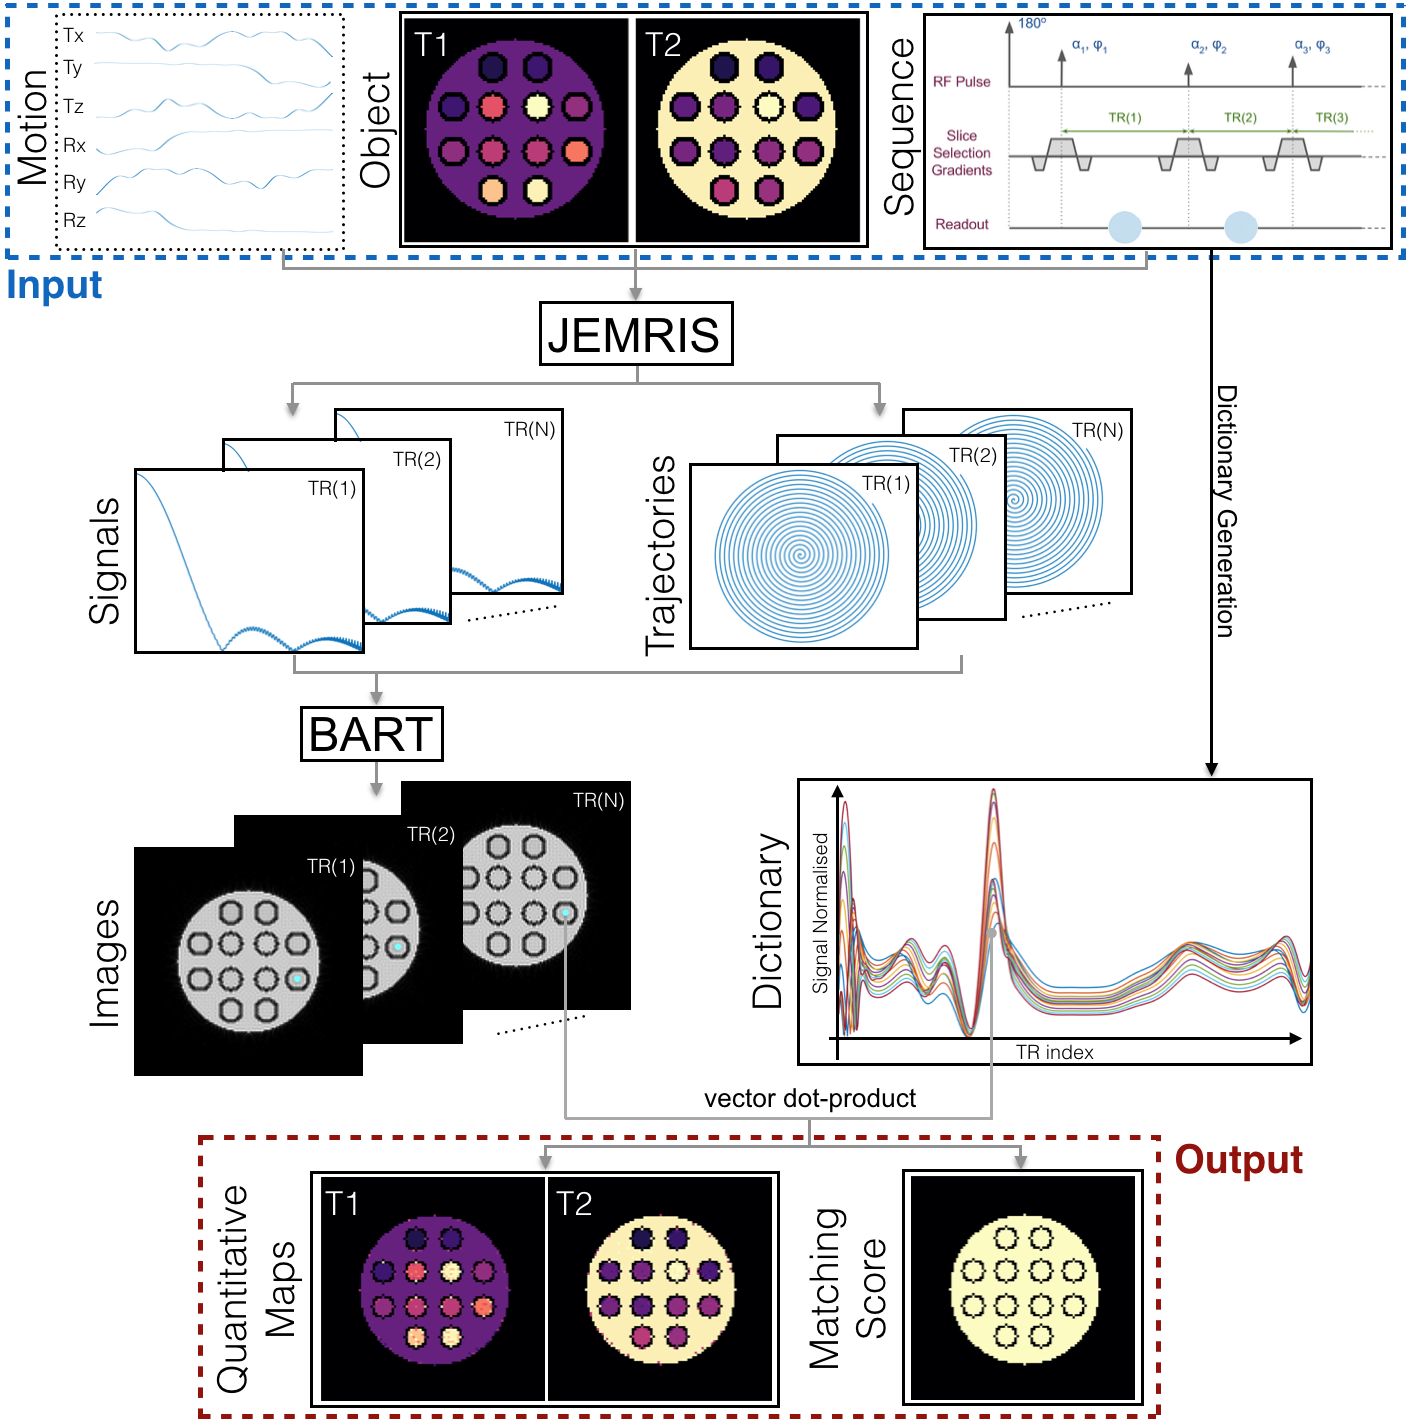
\includegraphics[angle=0,width=1\textwidth, keepaspectratio]{images/mrf/methodFramework}
    \caption{Image space simulation pipeline of a magnetic resonance fingerprinting experiment.
    The framework consists of three inputs: the digital phantom, the MR acquisition sequence and the motion trace. 
    The latter is shown here with dashed lines because it is an optional input parameter. 
    The open source MRI simulator JEMRIS is used to generate signals for each repetition period.
    Then, the BART toolbox is used to reconstruct the images.
    Separately, a dictionary of simulated signals is generated from first principles for a wide range of tissue properties.
    Finally, the quantitative maps are generated together with their corresponding pattern matching scores.}
    \label{fig:methodFramework}
\end{figure}

\hfill

The framework takes three inputs.
The first one is a geometric object which specifies the proton density and the $T_1$ and $T_2$ relaxation times at every spatial location.
The second is an inversion recovery rapid gradient-echo multi-pulse sequence with spiral readout (see Appendix \ref{chapterlabel2sec14}). 
For the dictionary generation part, I experimented with two types of sequences: \ac{bssfp} (see Appendix \ref{MRIBSSFP}) and \ac{fisp} (see Appendix \ref{MRIFISP}).
For the image space simulation part I have, so far, only simulated the \ac{bssfp} sequence.
The third input is the motion sequence where parameters for both translations and rotations can be specified.
These three inputs are then fed to JEMRIS which simulates the MR acquisition process and generates the signal for each repetition period of the multi-pulse sequence.
These signals, together with their corresponding k-space trajectory, are then fed into a software toolbox called BART \cite{Lustig2016} which reconstructs the images.
Separately, the same sequence is used to generate a database of signals, called `dictionary', for a wide range of relaxation parameters.

\hfill

The framework creates two outputs: the quantitative maps and the matching scores.
The former are created by first performing a voxel-wise pattern matching algorithm between all image space signals and all dictionary signals and then choosing the dictionary signal that gives the highest score as the most representative one for the voxel.
The latter are just the pattern matching scores showing how similar the two signals are.
More details related to the general MRF framework can be found in Appendix \ref{chapterlabel2sec22}.

\hfill

In the following sections I describe every part of our framework in more depth.
We start with the dictionary generation part as this is the first step in an MRF pipeline.
Next, I move on to explaining the image space simulations, together with the motion traces used for the experiments.
Finally, I explain the pattern matching algorithm used to create the quantitative maps.

\hfill

% % % % % % % % % % % % % % % % % % % % % % % % % % % % % % % % % % % % % % % % % % % % % % % % % % % % % % % % % % % % % % % % % % % % % % % % % % % % % % % % % % % % % % % % % % % % % % % % % % % % % % % % % % % % % % % % % % % % % % % % % % % % % % % % % % % % % % % % % % % % % % % % 
\subsection{Dictionary Generation}
\label{method:dictionary}

The first step in an MRF experiment is the creation of a dictionary of simulated signals for a wide variety of tissue properties.
This section presents an overview of the methods used for creating the database of signals for both a \ac{bssfp}-type sequence and a \ac{fisp}-type sequence.

\hfill

% \large \textbf{bSSFP Dictionary} \normalsize
\subsubsection{bSSFP Dictionary}

The \ac{bssfp} dictionary generation is based on the original implementation of the MRF sequence, where Ma et al. \cite{Ma2013} used an inversion-recovery balanced steady state free-precession sequence (see Figure~\ref{fig:sequencebSSFP}). 
The \ac{bssfp} sequence is a type of rapid multi-pulse gradient-echo pulse sequence. 
It is called `rapid' because the repetition time $T_R$ is shorter than both the longitudinal ($T_1$) and the transverse ($T_2$) relaxation times of most known tissue types.
Moreover, it uses balanced (fully rewound) gradients in every direction, thus effectively recovering the transverse magnetisation at the end of each $T_R$ period.

\hfill

\ac{bssfp} sequences are known to be highly sensitive to inhomogeneities in the main magnetic field. 
These inhomogeneities are caused by susceptibility variations or poor magnet shimming and give rise to `banding artifacts' in the final images \cite{Hargreaves2012}.
In spite of this, \ac{bssfp}-type sequences are used clinically today and are known commercially as: True-FISP, FIESTA, Balanced-FFE or True SSFP \cite{Hargreaves2012}.
These sequences are known to yield the highest signal among all the other rapid gradient-echo sequences and give a contrast of $T_2/T_1$ \cite{Scheffler2003}.

\begin{figure}[ht]
    \centering
    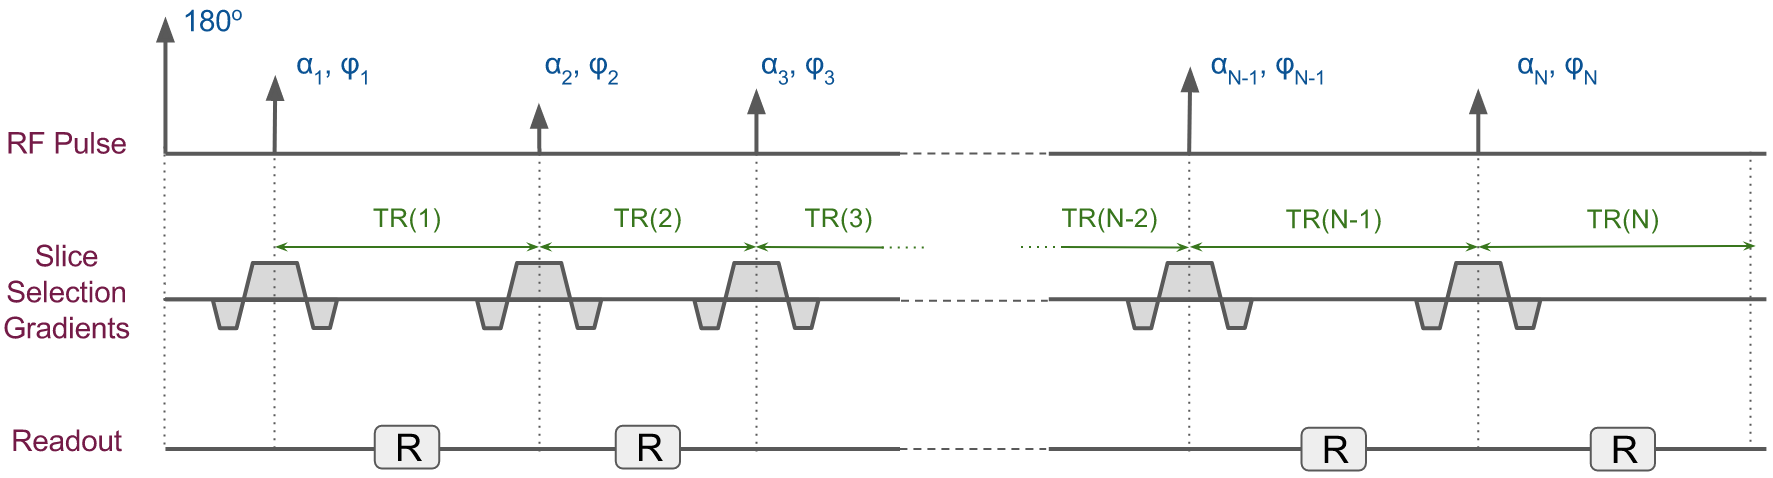
\includegraphics[angle=0,width=1\textwidth, keepaspectratio]{images/mrf/sequencebSSFP}
    \caption{The figure shows a simplified version of an IR-bSSFP sequence. 
    All gradients are fully balanced on every direction (they have a net moment of zero at the end of each repetition period) and readout is in the middle of each repetition period.}
    \label{fig:sequencebSSFP}
\end{figure}

\hfill

\large \textbf{Assumptions} \normalsize

To model the behaviour of a magnetisation vector with known relaxation times and proton density values in an MRF-\ac{bssfp} sequence, the following assumptions are made:

\begin{enumerate}
    \item The object for which I am modelling the magnetisation dynamics in the multi-pulse sequence is considered to be motionless.

    \item The effect of applying an RF pulse of flip angle $\alpha$ and phase angle $\phi$ was considered to be significantly shorter than the relaxation times $T_1$ and $T_2$ and was modelled as happening instantaneously.
    This allowed me to represent its effect as a rotation through the flip angle $\alpha$ about a chosen axis (e.g. the $x$-axis) and a change of coordinate system through the phase angle $\phi$ about the $z$-axis.
    This is called the "hard pulse approximation" and is detailed in Appendix~\ref{background:rfpulse}.
    
    \item The imaging gradients in this sequence are considered to be fully balanced (all the gradients have zero zeroth moment over each repetition period).
    Thus, any effect induced by the gradients is subsequently reversed by the rewinding gradients before the readout happens.
    I therefore neglected the effect of gradients on the magnetisation vector.

\end{enumerate}

\hfill

\large \textbf{Single Block Dynamics} \normalsize

In order to simulate the magnetisation dynamics in this multi-pulse sequence, 
%we first describe the effect of a single, arbitrarily chosen, $T_R$ block on a known magnetisation vector (see Figure~\ref{fig:sequencebSSFPOneBlock}).
I begin with the description of a single, arbitrarily chosen, $T_R$ block on a known magnetisation vector (see Figure~\ref{fig:sequencebSSFPOneBlock}).
The magnetisation vector immediately prior to the $i^{th}$ RF pulse is defined as:
\begin{equation}
    M^{-}_i \equiv \big[ M^-_{x_i} \, \,  M^-_{y_i} \, \, M^-_{z_i} \big]^T
\end{equation}
and immediately after the $i^{th}$ RF pulse as:
\begin{equation}
    M^{+}_i \equiv \big[ M^+_{x_i} \, \,  M^+_{y_i} \, \, M^+_{z_i} \big]^T
\end{equation}

\begin{figure}[ht]
    \centering
    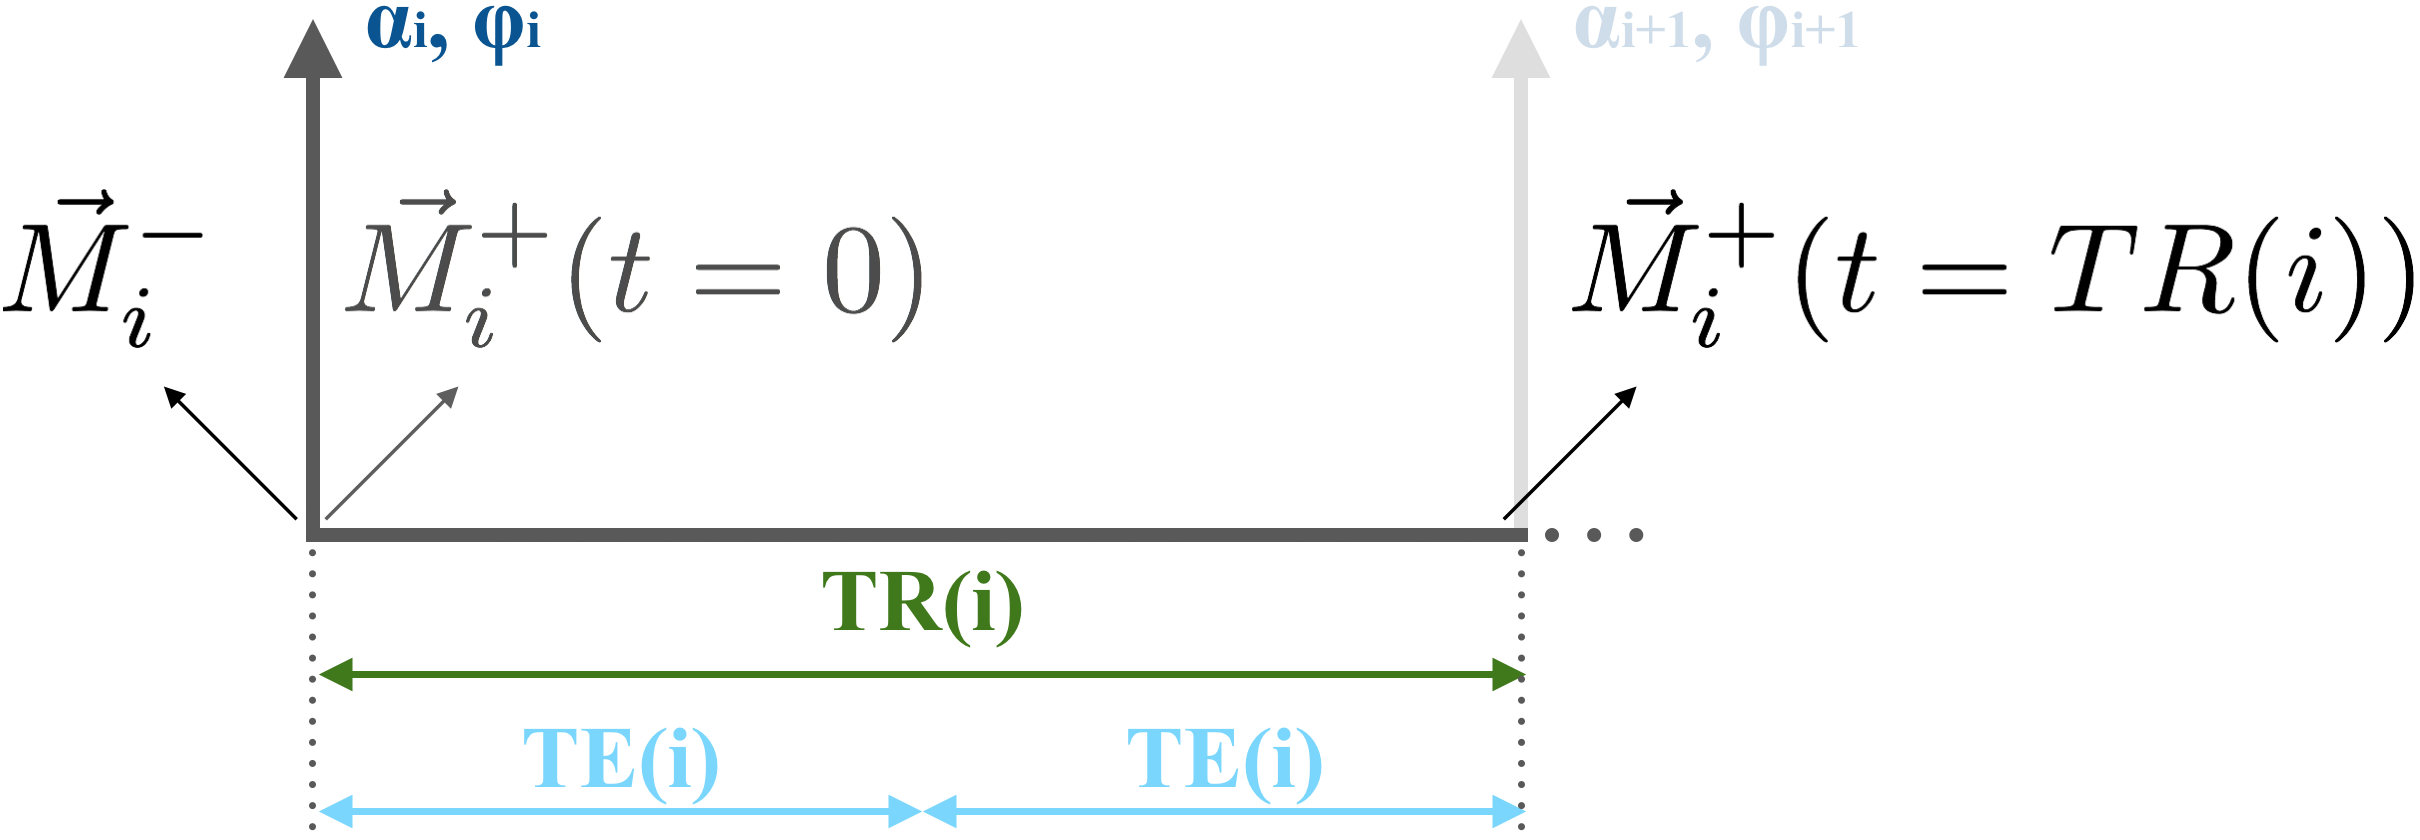
\includegraphics[angle=0,width=0.75\textwidth, keepaspectratio]{images/mrf/sequencebSSFPOneBlock}
    \caption{The figure shows a simplified version of an arbitrarily chosen repetition period block from the bSSFP sequence above.
    The magnetisation vector immediately prior to the $i^{th}$ RF pulse is denoted by $\vec{M}^-_i$ and the magnetisation vector immediately after the $i^{th}$ RF pulse is denoted by $\vec{M}^+_i$.
    The second magnetisation vector is formed as a result of the application of the $i^{th}$ RF pulse with flip angle $\alpha_i$ and phase angle $\phi_i$ on the $\vec{M}^-_i$ vector.
    Similarly, $\vec{M}^-_{i+1}$ and $\vec{M}^+_{i+1}$ are the magnetisation vectors immediately before and after the $(i+1)^{th}$ RF pulse.
    %The relationship between $\vec{M}^+_{i}$ and $\vec{M}^-_{i+1}$ is given by: $ \vec{M}^-_{i+1} = \vec{M}^+_{i}(t = TR(i))$, where $t \in [0, TR(i)]$ 
    }
    \label{fig:sequencebSSFPOneBlock}
\end{figure}

\textbf{RF Pulse.} 
The effect of an instantaneous RF pulse with flip angle $\alpha_i$ and phase angle $\phi_i$ links the two vectors through rotation matrices (see Appendix~\ref{app:rfpulse}):
\begin{equation}\label{eq:rfpulseequationbssfp}
    \begin{split}
        M^{+}_i & = R_{z}(\phi_i) R_{x}(-\alpha_i) R_{z}(-\phi_i) M^{-}_i \\
        \text{where:}         & \\
        & R_x(\alpha) = 
            \begin{bmatrix}
                1 &       0     &       0      \\
                0 & \cos(\alpha) & -\sin(\alpha) \\
                0 & \sin(\alpha) & \phantom{-}\cos(\alpha)
            \end{bmatrix} \\
        & R_z(\phi) = 
            \begin{bmatrix}
    	        \cos(\phi) & -\sin(\phi) & 0 \\
                \sin(\phi) & \phantom{-}\cos(\phi) & 0 \\
                    0   &      0     & 1
            \end{bmatrix}
    \end{split}
\end{equation}

\hfill

\textbf{Relaxation.} 
Next, the magnetisation vector will begin the process of returning to its equilibrium state.
This phenomenon is governed by the $T_1$ and $T_2$ relaxation times of the tissue being modelled and can be described using matrix notation (more details in Appendix~\ref{chapterlabel2sec1Bloch}).
In the rotating reference frame (after demodulating with the Larmor frequency $\omega_0$), this phenomenon can be described as:

\begin{equation}
    M^{+}_i (t)  = D(t) M^{+}_i (0) + C(t)
\end{equation}
where
\begin{equation}\label{eq:dmatrix}
    D ( t ) = \left[
    \begin{array}{c c c}
          E_2(t) &     0      &     0 \\
          0      & E_2(t) &     0 \\
          0      &     0      & E_1(t)
    \end{array}
    \right] \, \, \text{,  } \, 
    C ( t ) = \left[
    \begin{array}{c}
        0 \\
        0 \\
    M_0(1 - E_1(t))
    \end{array}
    \right]
\end{equation}

and where $E_1(t) \equiv e^{-t/T_1}$, $E_2(t) \equiv e^{-t/T_2}$ and
$t \in [0, T_R(i)]$.

\hfill

\textbf{Off-resonance.} 
In the case where static field inhomogeneities $\Delta B$ are present, the phase of the magnetisation vector will change over a given repetition time period. 
This phase is determined by $\beta(t) = \gamma \Delta B t = \Delta \omega t = 2\pi \Delta \nu t$ during any $T_R$ block.
To model the behaviour of phase accrual, an instantaneous rotation about the $z$ axis of the magnetisation vector is used.
This can be mathematically represented as:

\begin{equation}
    M^{+}_i (t)  = R_z(\beta(t)) M^{+}_i (0)
\end{equation}

where the rotation matrix $R_z$ has been previously described.
%and $\beta(t) = 2\pi \, \, \Delta \nu \, \, t$ is the accumulated phase due to off-resonance frequency $\Delta \nu$ at time $t$ during the $i^{th}$ repetition period. 
%Again, we can choose $t = T_{E_i}$ or $t = T_{R_i}$ to calculate the magnetisation vector components at the echo time or at the end of a repetition period, respectively.

\hfill

\large \textbf{Multiple Blocks Dynamics} \normalsize

The extension from single block simulations to multi-pulse simulations is straightforward.
The resulting magnetisation vector at the end of the $i^{th}$ repetition period becomes the magnetisation vector immediately prior to the $(i+1)^{th}$ RF pulse, where the process is repeated with the sequence properties corresponding to the following block:

\begin{equation}
    M^{-}_{i+1} = D\big(T_R(i)\big) R_z\big(\beta(T_R(i))\big) \big( R_{z}(\phi_i) R_{x}(-\alpha_i) R_{z}(-\phi_i) M^{-}_i \big) + C\big(T_R(i)\big)
\end{equation}

where $M^{-}_1 = M_0 \hat{x}$ and $i \in [1, N_{pulses}]$.

\hfill

% The magnetisation vector components at echo time can be calculated for every $T_R$ block and the signal for a single tissue type in a multi-pulse sequence can be retrieved.
% These events can now be linked together to calculate the magnetisation vector at time $t$ after the $i^{th}$ RF pulse:

% These three events, RF pulse, relaxation and off-resonance effects, fully describe the magnetisation dynamics of a spin ensemble with equilibrium magnetisation $M_0$, relaxation constants $T_1$ and $T_2$, and with off-resonance frequency $\Delta \nu$.
% These events can now be linked together to calculate the magnetisation vector at time $t$ after the $i^{th}$ RF pulse:
% \begin{equation}
%     M^{+}_i (t) = D(t) R_z(\beta(t)) \big( R_{z}(\phi_i) R_{x}(-\alpha_i) R_{z}(-\phi_i) M^{-}_i \big) + C(t)
% \end{equation}

\large \textbf{Dictionary} \normalsize

In order to create a dictionary of signals in a multi-pulse IR-\ac{bssfp} sequence, the previously described process is repeated for a range of tissue properties.
More specifically, every signal is associated with a `tissue tuple':
$(T_{1_j}, T_{2_j}, \Delta f_{j})$, with $j \in [1, M]$, where $M$ is the total number of tuples.
Hence, the dictionary is creating a function relationship between tissue properties and signals.

\hfill

The dictionary was created in MATLAB using a vectorised version of the previously described process.
The speed of this method comes from the fact that the magnetisation vector components of all tissue types are calculated simultaneously, for every $T_R$ period.
For this, I start by defining a $3 \times M$ matrix for the $M_x, \, M_y, \, M_z$ components of the magnetisation vector for all $M$ tissue types immediately before the $i^{th}$ RF Pulse:
\begin{equation}
    M^{-}_i = 
    \begin{bmatrix}
        M_{ix_1} & M_{ix_2} & \dots & M_{ix_M} \\
        M_{iy_1} & M_{iy_2} & \dots & M_{iy_M} \\
        M_{iz_1} & M_{iz_2} & \dots & M_{iz_M}
    \end{bmatrix}
\end{equation}

To flip the magnetisation vectors of all the tissue types, the RF pulse matrix is precomputed for the current repetition period:
\begin{equation}
        R_{\phi_i}(\alpha_i) = R_{z}(\phi_i) R_{x}(-\alpha_i) R_{z}(-\phi_i)
\end{equation}
and then applied to the previously defined $3 \times M$ matrix of magnetisation vector components:
\begin{equation}
    M^{+}_i(0) = R_{\phi_i}(\alpha_i) \, \, M^{-}_i
\end{equation}

For the off-resonance effects, the process is split in two.
Two $3 \times M$ matrices are created to represent the effect of rotation about the z-axis for all possible $\beta_j(t) = 2\pi \Delta \nu_j \, t$ \big(with $j \in [1, M]$ \big) off-resonance angles.
Mathematically, this is given by:
\begin{equation}
    M^{+}_i (t) = R_{\Delta \nu_1}(t) \, \odot \, M^{+}_i(0) + R_{\Delta \nu_2}(t)  \, \odot \, M^{+}_i(0)^{(p)}
\end{equation}

where $\odot$ denotes component-wise multiplication, and:

\begin{equation}
    R_{\Delta \nu_1}(t)  = \begin{bmatrix} \phantom{-}\cos(\beta_{1}(t) ) & \phantom{-}\cos(\beta_{2}(t) ) & \dots & \phantom{-}\cos(\beta_{M}(t) ) \\
    \phantom{-}\cos(\beta_{1}(t) ) & \phantom{-}\cos(\beta_{2}(t) ) & \dots & \phantom{-}\cos(\beta_{M}(t) ) \\
    1    &        1   & \dots &  1
    \end{bmatrix}
\end{equation}

\begin{equation}
    R_{\Delta \nu_2}(t)  = \begin{bmatrix} -\sin(\beta_{1}(t) ) & -\sin(\beta_{2}(t) ) & \dots & -\sin(\beta_{M}(t) ) \\
    \phantom{-}\sin(\beta_{1}(t) ) & \phantom{-}\sin(\beta_{2}(t) ) & \dots & \phantom{-}\sin(\beta_{M}(t) ) \\
    0     &      0      & \dots &      0
    \end{bmatrix}
\end{equation}

\begin{equation}
\begin{split}
    M^{+}_i(0) = &
    \begin{bmatrix}
        M^{+}_{ix_1}(0) & M^{+}_{ix_2}(0) & \dots & M^{+}_{ix_M}(0) \\
        M^{+}_{iy_1}(0) & M^{+}_{iy_2}(0) & \dots & M^{+}_{iy_M}(0) \\
        M^{+}_{iz_1}(0) & M^{+}_{iz_2}(0) & \dots & M^{+}_{iz_M}(0)
    \end{bmatrix} \\
    = & \, \, R_{\phi_i}(\alpha_i) \, \, M^{-}_i \text{ (as previously defined)}
\end{split}
\end{equation}

\begin{equation}
\begin{split}
    M^{+}_i(0)^{(p)} = &
    \begin{bmatrix}
        M^{+}_{iy_1}(0) & M^{+}_{iy_2}(0) & \dots & M^{+}_{iy_M}(0) \\
        M^{+}_{ix_1}(0) & M^{+}_{ix_2}(0) & \dots & M^{+}_{ix_M}(0) \\
        M^{+}_{iz_1}(0) & M^{+}_{iz_2}(0) & \dots & M^{+}_{iz_M}(0)
    \end{bmatrix} \\
    & \text{ (Obs: lines 1 and 2 have been permuted)}
\end{split}
\end{equation}

For the relaxation effects, two $3 \times M$ matrices are built to account for all M combinations of $T_1$ and $T_2$ decay rates:
\begin{equation}
    M^{+}_i(t) = D(t)  \, \odot \, M^{+}_i(0) + C(t) 
\end{equation}

where, again, $\odot$ denotes component-wise multiplication, and:

\begin{equation}
    D(t)  = 
    \begin{bmatrix}
        E_{2_1}(t)  & E_{2_2}(t)  & \dots & E_{2_M}(t)  \\
        E_{2_1}(t)  & E_{2_2}(t)  & \dots & E_{2_M}(t)  \\
        E_{1_1}(t)  & E_{1_2}(t)  & \dots & E_{1_M}(t)  
    \end{bmatrix}
\end{equation}

and

\begin{equation}
    C(t)  = 
    \begin{bmatrix}
        0 & 0 & \dots & 0 \\
        0 & 0 & \dots & 0 \\
        1 - E_{1_1}(t)  & 1- E_{1_2}(t)  & \dots & 1- E_{1_M}(t)  
    \end{bmatrix} 
\end{equation}

where $E_{1_j}(t) \equiv e^{-t/T_{1_j}}$ and $E_{2_j}(t) \equiv e^{-t/T_{2_j}}$, with $j \in [1, M]$.

\hfill 

This process is then repeated, in order, for all repetition times in the sequence.
At the end, a dictionary of M signals, each with N time points is constructed.
For completion, I store all 3 components of the magnetic moment vectors, thus having an $M \times N \times 3$ dictionary matrix.
Pseudocode for the created algorithms can be found in Appendix~\ref{appendixlabel1}.

\hfill

\subsubsection{FISP Dictionary} 
\label{method:fispdictionary}

The \ac{fisp} dictionary generation is based on a more recent implementation of the MRF sequence, where Jiang et al. \cite{Jiang2015} used an inversion-recovery fast imaging with steady-state precession sequence (see Figure~\ref{fig:sequenceFISP}).
Similar to \ac{bssfp}, \ac{fisp} is also a type of rapid multi-pulse gradient-echo sequence.
However, in contrast with the previous sequence, \ac{fisp} uses an unbalanced gradient in one or multiple gradient directions, thus `spoiling' the transverse magnetization prior to the next RF pulse \cite{Hargreaves2012}.
Gradient spoiling does not effectively null the transverse magnetisation, so then both the longitudinal and the transverse magnetisation components will contribute to the signal in the next cycle.

\begin{figure}[ht]
    \centering
    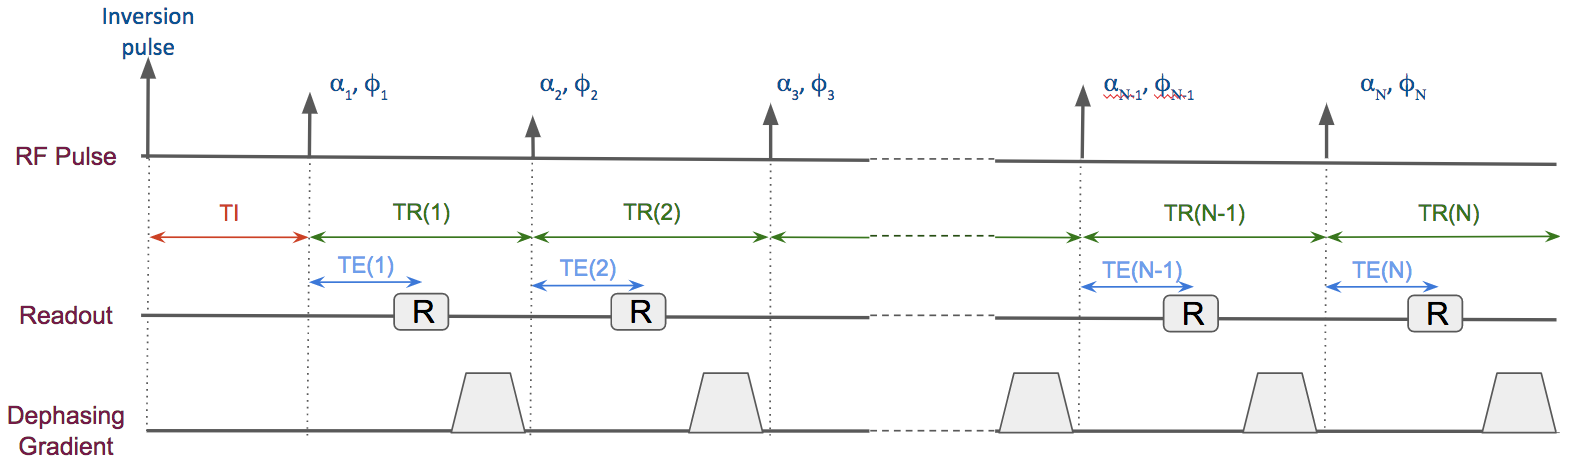
\includegraphics[angle=0,width=1\textwidth, keepaspectratio]{images/mrf/sequenceFISP}
    \caption{The figure shows a simplified version of an inversion recovery fast imaging with steady state precession sequence. 
    Unlike \ac{bssfp}, a \ac{fisp} sequence contains an unbalanced `spoiler' gradient in each each repetition period.
    Otherwise, all other gradients are fully balanced in every direction.
    Here, $N$ represents the total number of RF pulses.}
    \label{fig:sequenceFISP}
\end{figure}

\hfill

\ac{fisp}-type sequences are used in MR imaging due to their fast imaging characteristics and their immunity to the banding artefacts commonly seen in fully balanced steady state sequences. 
%As with \ac{bssfp}, the signal in these types of sequences is a function of $T_2/T_1$ \cite{Hargreaves2012}. 
%\ac{fisp}-type sequence yield a lower signal than in \ac{bssfp} and 
Commercially, \ac{fisp}-type sequences are known as: FE, FFE, GRASS, GRE, \ac{fisp}, FAST \cite{Hargreaves2012}.
These sequences are known to yield a lower signal magnitude than balanced sequences, while keeping a similar signal contrast of $T_2/T_1$ \cite{Hargreaves2012}.

\hfill

\large \textbf{Assumptions} \normalsize

In order to simulate the behaviour of a magnetisation vector with known relaxation times and proton density values in an MRF-\ac{fisp} sequence, single isochromat Bloch equations are no longer applicable.
Due to the presence of a strong dephasing gradient and repetition times shorter than the transverse relaxations of most tissue types \big($T_R \leq T_2$\big), the transverse magnetisation will not be destroyed, but completely dephased across a voxel.
To model this, an algorithm called the \ac{epg} \cite{Hennig1988} \cite{Hennig1991} was used.

\hfill 

The \ac{epg} formalism \cite{Hennig1988} \cite{Hennig1991} \cite{Weigel2015} is used to simulate signals obtained from a wide variety of MRI pulse sequences \cite{Malik2017}.
% EPG has been used for a variety of applications such as:
% characterization of RF spoiling in gradient echo sequences (4,5), 
% analysis of echo amplitudes in turbo spin echo (TSE) sequences (6–9), 
% diffusion effects (12), and 
% characterizing signal evolution in sequences used for relaxometry (13–16).
Similar to the Bloch equations approach, \ac{epg} characterizes a given sequence through the effects of RF pulses, relaxation constants, and dephasing due to gradients or inhomogeneities in the main magnetic field.
% However, in this formalism large groups of spins are represented as a compact Fourier basis set of $F_k$ and $Z_k$ coefficients.
% However, unlike the previous approach, EPG describes a spin system as a discrete set of phase states (or, `configuration states') \cite{Hennig1988}.
% These states appear as a consequence of 
To model the behaviour of a spin ensemble 
%with known relaxation times and proton density values 
in a single-voxel MRF-\ac{fisp} sequence, the following assumptions were made:
% This algorithm works under certain assumptions which we enumerate here:

%Bloch equations can be used, but a large number of isochromats needs to be simulated to achieve accuracy.
% For this, a different approach was used, called the Extended Phase Graph formalism \cite{Hennig1988} \cite{Hennig1991}.

\begin{enumerate}

    \item The object for which I am modelling the magnetisation dynamics in the multi-pulse sequence is considered to be motionless.

    \item The tissue being modelled is represented by a single voxel with uniform density of magnetisation, characterised by a single set of relaxation parameters and spin density values.
    
    \item The 1D voxel has dimension in the same direction as the applied gradient, where one edge of the voxel is considered to be the `isocentre'.
    Gradient areas are quantized into units that give a phase twist of one cycle ($2\pi$), such that the amount of dephasing induced by one application of the gradient is ranging from $[0, 2\pi]$. 
    Moreover, for improved visualisation and pictorial understanding, I presume that the gradient is in the z-direction.

    \item The `spoiling' gradient used in this sequence has the same amplitude and duration in every repetition period.
    Thus, the gradient induces the same amount of dephasing across the voxel during each of its applications.
    %a fixed time period $\Delta t$ at the end of each repetition period.
    
    \item The effect of applying an RF pulse of flip angle $\alpha$ and phase angle $\phi$ was considered to be significantly shorter than the relaxation times $T_1$ and $T_2$ and was modelled as happening instantaneously.
    This allowed me to represent its effect as a rotation through the flip angle $\alpha$ about a chosen axis (e.g. the $x$-axis) and a change of coordinate system through the phase angle $\phi$ about the $z$-axis.
    This is called the hard pulse approximation and is detailed in Appendix~\ref{background:rfpulse}.

\end{enumerate}

\hfill

\large \textbf{Extended Phase Graph Formalism} \normalsize

In this section explains the main ingredients behind the \ac{epg} formalism, starting from a simple example of a fully relaxed spin system.
The extended phase graph formalism is a tool for understanding MR signal progression and echo formation in a wide variety of MR sequences.
In \ac{epg}, the full state of the signal across a voxel is represented by a small number of coefficients.
These coefficients encode the distribution of the isochromat population into different Fourier basis functions.
These basis functions are either a set of transverse basis functions called $\bm{F_k}$ and $\bm{F_{-k}}$ or longitudinal basis functions called $\bm{Z_k}$.

\hfill

Mathematically, these configuration states are related to
%form a Fourier pair with 
the complex transverse magnetisation $M_{+}$ and longitudinal magnetisation $M_z$ \cite{Hennig1991} through:
\begin{equation}
\begin{split}
    F_{k}  & = \int_0^1 M_{+}(z) e^{- i 2\pi k z} dz \\ %& \Longleftrightarrow M_{+}(z) = \int_{- \infty}^{+ \infty}  F_{k} e^{+ i 2\pi k z} dk \\
    F_{-k} & = \int_0^1 M_{-}(z) e^{- i 2\pi k z} dz \\ %& \Longleftrightarrow M_{-}(z) = \int_{- \infty}^{+ \infty}  F_{-k} e^{+ i 2\pi k z} dk \\
    Z_{k} & = \int_0^1 M_{z}(z) e^{- i 2\pi k z} dz %& \Longleftrightarrow M_{z}(z) = \int_{- \infty}^{+ \infty} Z_{k} e^{+ i 2\pi k z} dk
\end{split}    
\end{equation}
where z is the voxel dimension and is in the $[0,1]$ range (without loss of generality) and $M_+ = (M_-)^*$.
The $F_{k}$ and $F_{-k}$ states can be thought of as a two counter-rotating isochromat populations \cite{Brown}.

\hfill

\textbf{The $\bm{F_0}$ and $\bm{Z_0}$ configuration states}

% In this section we explain the main ingredients behind the EPG formalism, starting from a simple example of a fully relaxed spin system.
%In order to model the behaviour of a spin ensemble with known relaxation times and proton density values in a single-voxel MRF-\ac{fisp} sequence, 
%In order to simulate the magnetisation dynamics in this multi-pulse sequence, 
%we begin with the description of a single $T_R$ block.
%In order to 
% To simplify things even further, we begin with the thermal equilibrium case, where the spin ensemble is fully relaxed and the magnetic moment vectors have the same direction as the main magnetic field (here considered to be $\hat{z}$).
At thermal equilibrium, an isochromat ensemble is fully relaxed and the magnetic moment vectors have the same direction as the main magnetic field (here considered to be $\hat{z}$).
This state in which the spin system is initially found is called a $\bm{Z_0}$ configuration \cite{Weigel2015} \cite{Scheffler1999} \cite{Hennig1991}.
The coefficient for this state is equal to $\bm{1}$ as the entire population of the imaginary spin ensemble is found in this configuration.
Pictorially, the $\bm{Z_0}$ state is shown in Figure~\ref{fig:Z0F0states} a) where I chose to represent 100 uniformly distributed isochromats along the voxel dimension.

\hfill

The application of an instantaneous $\pi/2$ excitation pulse on this configuration has the effect of `flipping' the entire isochromat ensemble in the transverse plane.
This new configuration is known as the $\bm{F_0}$ state \cite{Weigel2015} \cite{Scheffler1999} \cite{Hennig1991} and is graphically shown in Figure~\ref{fig:Z0F0states} b).
The $\bm{F_0}$ configuration is an important concept in the \ac{epg} formalism as it represents coherent transverse magnetisation and it is the cause of echo generation.
% 
% \hfill
% 
% The isochromat ensemble can `flip' back and forth between the two states by the application of the same instantaneous $\pi/2$ pulse.

\begin{figure}[H]
    \centering
    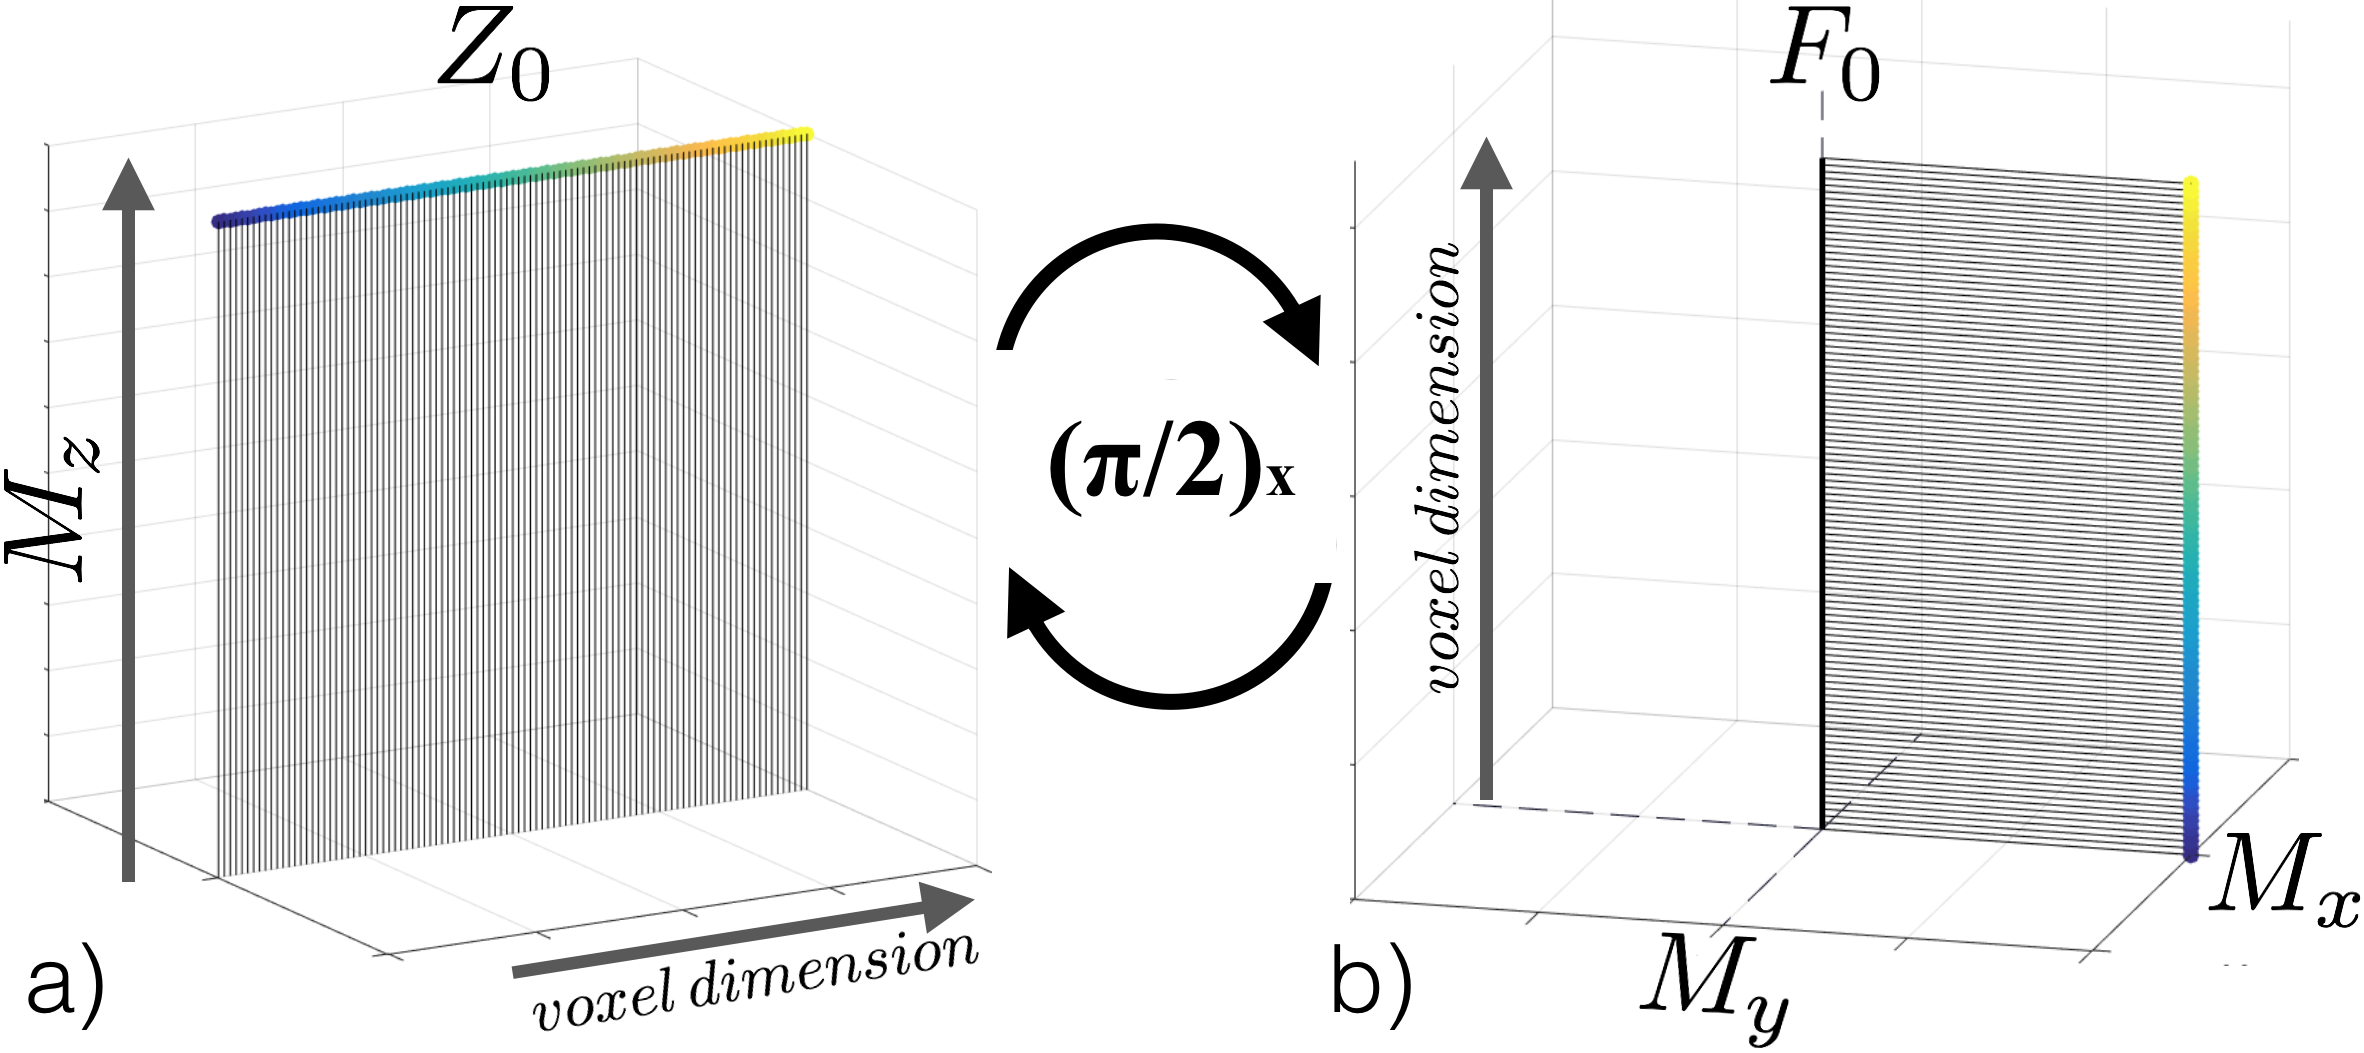
\includegraphics[angle=0,width=0.65\textwidth, keepaspectratio]{images/mrf/Z0F0states}
    \caption{The figure shows a pictorial representation of a single 1D voxel with uniform density of magnetisation.
    a) $\bm{Z_0}$ is a configuration in which the isochromat ensemble is characterised by spins lying along $M_z$.
    b) $\bm{F_0}$ is a configuration in which the isochromat ensemble is characterised by coherent transverse magnetisation.
    An instantaneous $\pi/2$ excitation pulse can `flip' the isochromat ensemble back and forth between the two states.
    It is important to note that a $(\pi/2)_x$ RF pulse applied on the $\bm{F_0}$ state will cause the isochromat ensemble to be pointing in the $- \hat{z}$ direction instead of the $+ \hat{z}$ direction it was initially found.
    However, this is still considered a $\bm{Z_0}$ configuration.
    }
    \label{fig:Z0F0states}
\end{figure}


\begin{figure}[H]
    \centering
    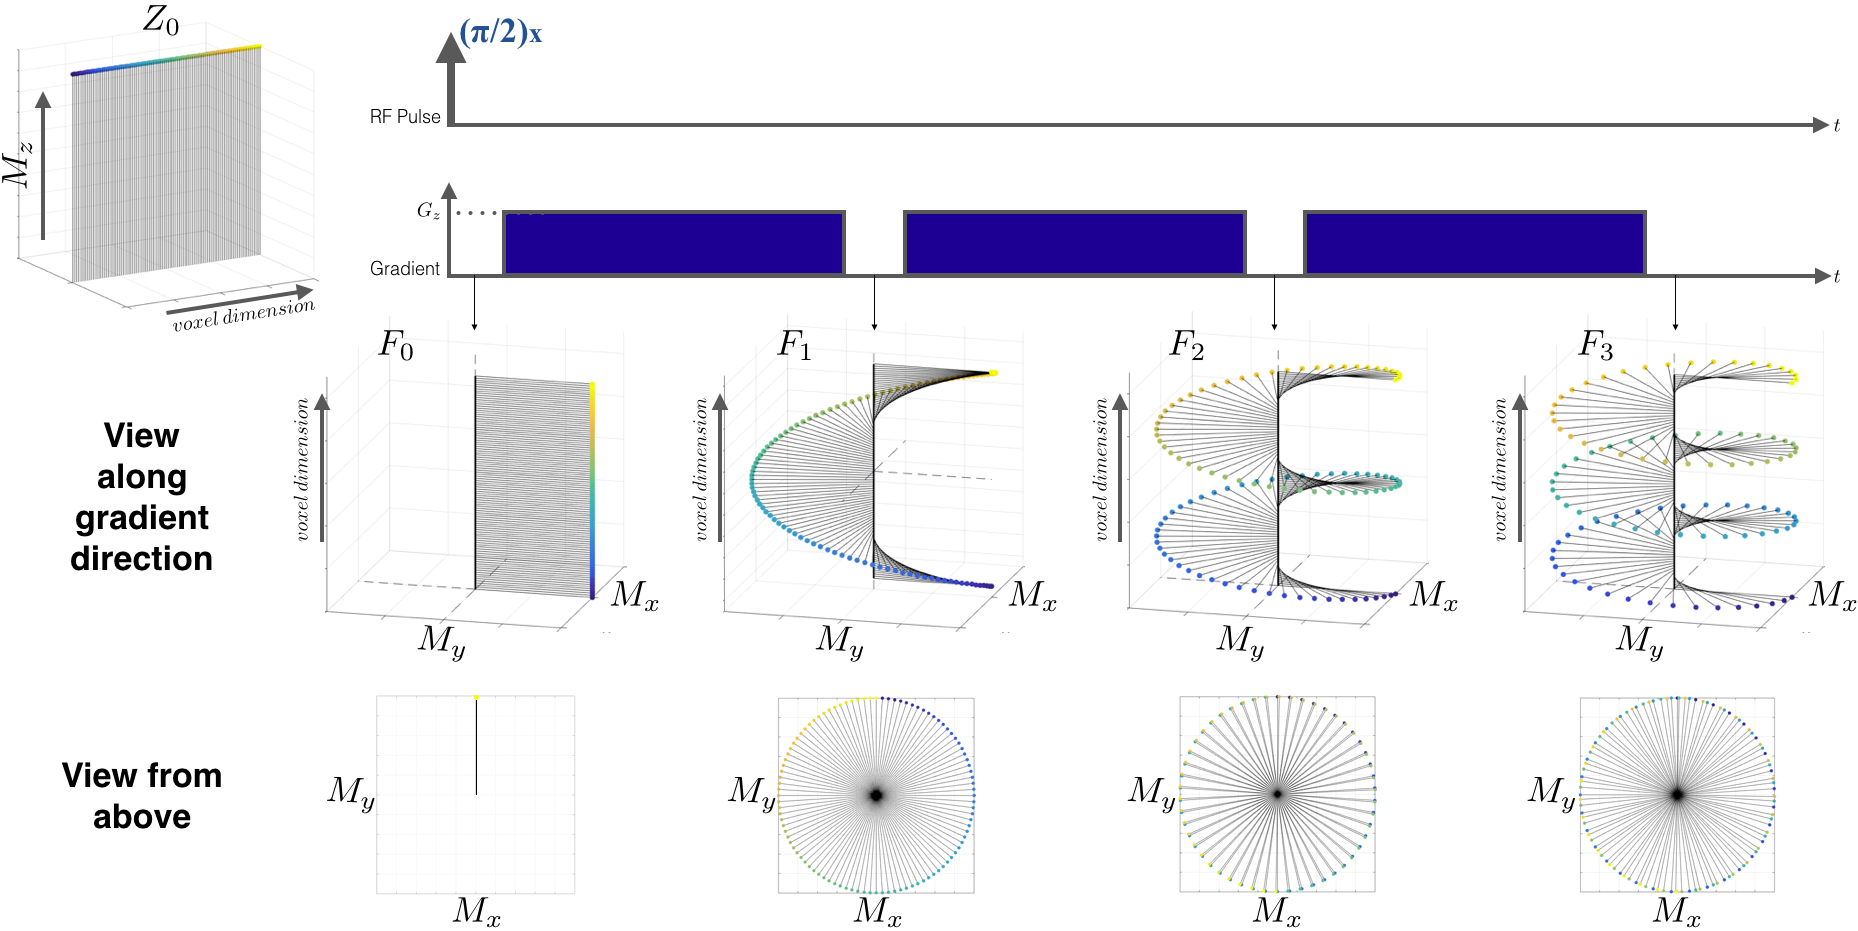
\includegraphics[angle=90,width=0.7\textwidth, keepaspectratio]{images/mrf/effectOfGradsEPG}
    \caption{Pictorial representation of an isochromat ensemble experiencing an ideal instantaneous $(\pi/2)_x$ RF pulse and dephasing induced by a gradient.
    This spin system is found in a 1D voxel whose dimension in along the same direction as the applied gradient (here, the $\hat{z}$ direction is considered) and which is positioned such that one edge of the voxel is at the `isocentre'. The isochromats found at the opposite edge accrue a phase of $2\pi$ after the application of this gradient.
    Every time the gradient is applied the spin system dephases further into a new configuration here represented as discrete states: $\bm{F_k}$.}
    \label{fig:effectOfGradsEPG}
\end{figure}

% % % % % % % % % % % % % % % % % % % % 
\textbf{The effect of a constant gradient on the isochromat ensemble} 

The application of a constant gradient introduces a linearly position-dependent off-resonance Larmor frequency on the isochromat ensemble along its axis (which is the same as the voxel dimension, as stated in the assumptions).
This can be seen in Figure~\ref{fig:effectOfGradsEPG} where after the first application of the gradient the spin system is now dephased.
This dephased configuration can be conceptually represented as an evenly distributed collection of magnetisation vectors called $\bm{F_1}$ \cite{Hennig1988} \cite{Scheffler1999}, where $\bm{k=1}$ represents one cycle of phase.
% Let us now introduce a dephasing gradient in the $\hat{z}$ direction (the 1D voxel's direction) that obeys the assumptions we previously described.
% This gradient induces phase accrual on the isochromat ensemble such that the isochromat found at one edge of the voxel is positioned at the `isocentre', while the isochromat found at the opposite edge experiences $2\pi$ dephasing.
% In fact, the off-resonance frequency increases linearly with the distance from the assumed `isocentre'.

\hfill

Each further application of the gradient increases the amount of dephasing experienced by the spin system with multiples of $2\pi$.
This can be seen in Figure~\ref{fig:effectOfGradsEPG} where each new application of the gradient `shifts' the spin system into a different configuration state.
These dephased configuration states are called $\bm{F_k}$, where $k$ represents the amount of $2\pi$ dephasing experienced by the spin ensemble.

\hfill

% % % % % % % % % % % % % % % % % % % % 
\textbf{The effect of an RF pulse on the isochromat ensemble} 

The application of an RF pulse of arbitrary flip angle $\alpha$ and phase angle $\phi$ on a dephased isochromat ensemble mixes the populations of spins among configurations.
This effect is best explained through equation \ref{eq:rfpulseequationbssfp}, which says that the magnetisation vectors immediately after the RF pulse are related to those immediately before the RF pulse through a rotation matrix (relaxation effects are neglected as the RF pulse is assumed to be instantaneous).
For completion, I rewrite equation \ref{eq:rfpulseequationbssfp} here:

\begin{equation}
    \begin{bmatrix} 
    M_x \\
    M_y \\
    M_z
    \end{bmatrix}^+ = 
        R_{\phi}(\alpha)
    \begin{bmatrix} 
    M_x \\
    M_y \\
    M_z
    \end{bmatrix}^-
\end{equation}
where, as before, superscript $+$ denotes `immediately after RF pulse' and superscript $-$ denotes 'immediately before RF pulse'.

\hfill

In complex notation, where $M_+ \equiv M_x + i M_y$,  $M_- \equiv M_x - i M_y$ and $M_- = (M_+)^*$ this becomes:

\begin{equation}\label{eq:magnbeforestates}
    \begin{bmatrix} 
    M_+ \\
    M_- \\
    M_z
    \end{bmatrix}^+ = 
        T_{\phi}(\alpha)
    \begin{bmatrix} 
    M_+ \\
    M_- \\
    M_z
    \end{bmatrix}^-
\end{equation}
where 
\begin{equation}\label{eq:woessnerFn2}
    T_{\phi}(\alpha) = 
    \begin{bmatrix}
        cos^2(\alpha/2) & e^{2i\phi} sin^2(\alpha/2) & - i e^{i \phi} sin(\alpha) \\
        e^{-2i\phi} sin^2(\alpha/2) & cos^2(\alpha/2) & i e^{-i \phi} sin(\alpha) \\
        - i/2 e^{-i \phi} sin(\alpha) & i/2 e^{i \phi} sin(\alpha) & cos \alpha
    \end{bmatrix}
\end{equation}

\hfill

% A completely dephased isochromat ensemble is rotated through an angle by the applied instantaneous RF pulse.
% This is seen in Figure~\ref{fig:RFpulseeffect} where we chose $\phi = 0$.

% \begin{figure}[ht]
%     \centering
%     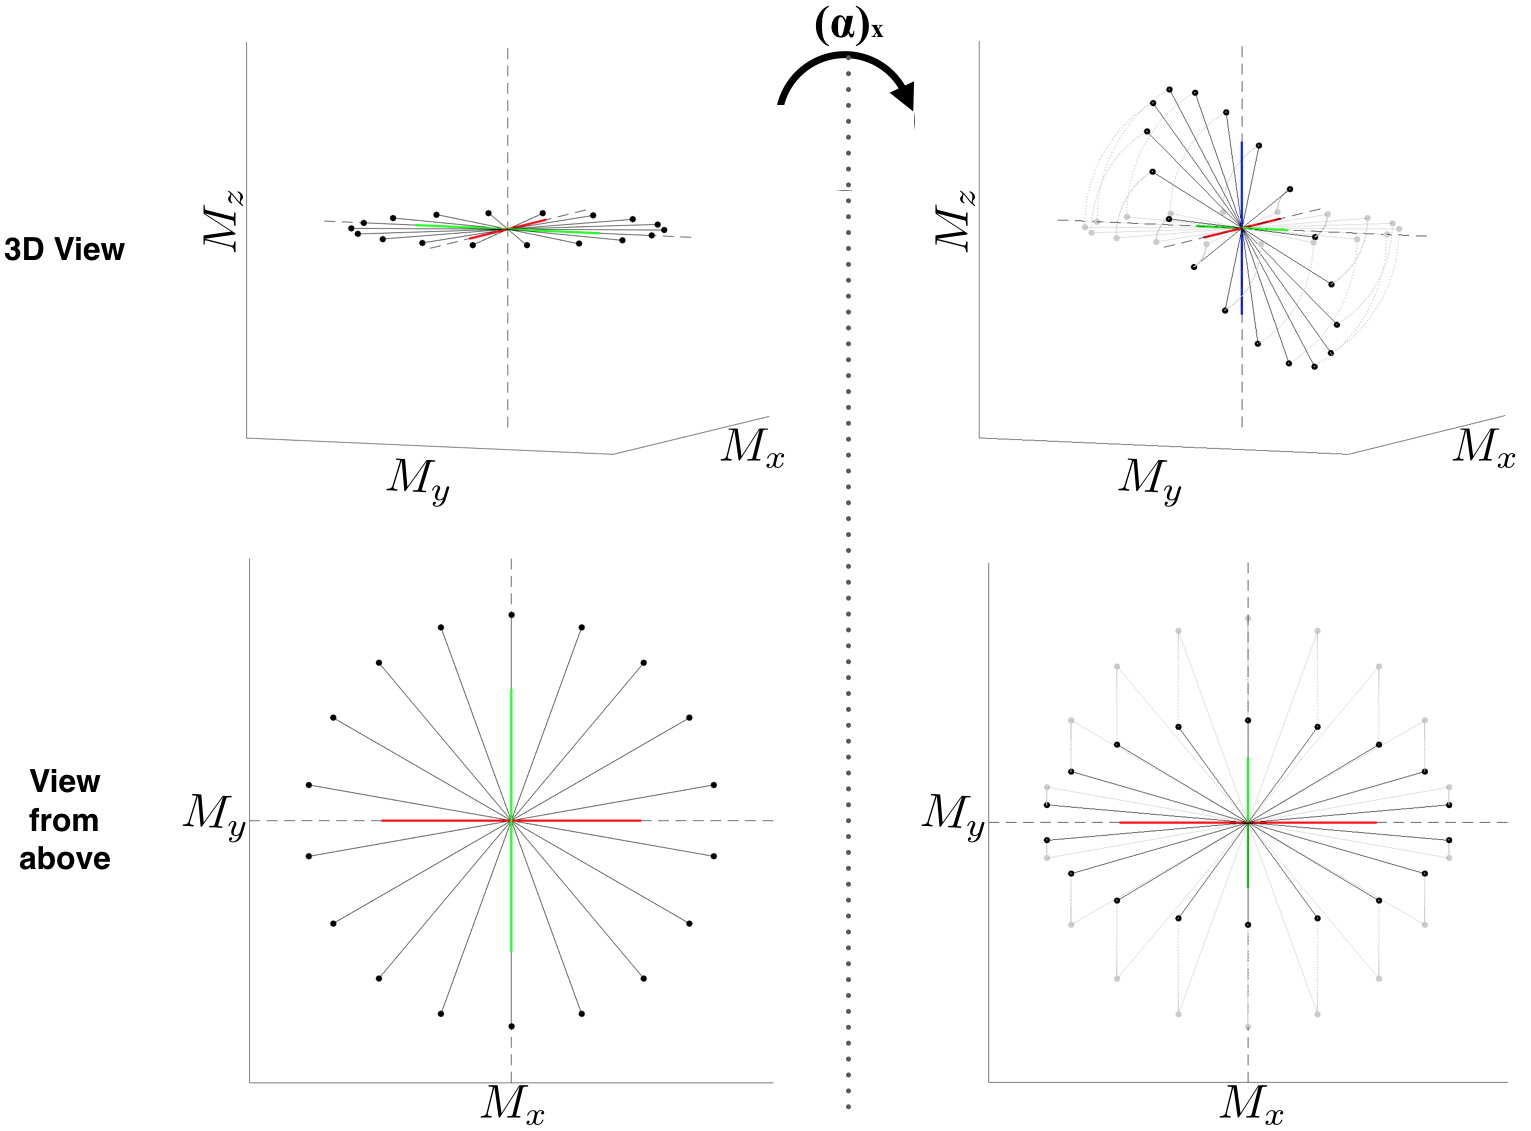
\includegraphics[angle=0,width=1\textwidth, keepaspectratio]{images/mrf/RFpulseeffect}
%     \caption{Pictorial representation of a completely dephased isochromat ensemble experiencing an ideal instantaneous $(\alpha)_x$ RF pulse.}
%     \label{fig:RFpulseeffect}
% \end{figure}
The transition to configuration states is straight forward, as the complex magnetisation vectors can be easily replaced with the partition states (the details of which are found in Hennig \cite{Hennig1991}).
Equation \ref{eq:magnbeforestates} becomes:

\begin{equation}\label{eq:magnafterstates}
    \begin{bmatrix} 
    F_{k} \\
    F_{-k} \\
    Z_{k}
    \end{bmatrix}^+ = 
        T_{\phi}(\alpha)
    \begin{bmatrix} 
    F_{k} \\
    F_{-k} \\
    Z_{k}
    \end{bmatrix}^-
\end{equation}

\hfill 

Expanding equation \ref{eq:magnafterstates} into its components yields:
\begin{equation}\label{eq:woessner}
\begin{split}
    F_{k}^+ &= F_{k}^- cos^2(\alpha/2) + e^{2i\phi} F_{-k}^- sin^2(\alpha/2)  - i e^{i \phi} Z_{k}^- sin(\alpha)  \\
    F_{-k}^+ &=  e^{-2i\phi} F_{k}^- sin^2(\alpha/2) + F_{-k}^- cos^2(\alpha/2) + i e^{-i \phi} Z_{k}^- sin(\alpha) \\
    Z_{k}^+ &= - i/2 e^{-i \phi} F_{k}^- sin(\alpha) + i/2 e^{-i \phi} F_{-k}^- sin(\alpha) + Z_{k}^- cos(\alpha) 
\end{split}
\end{equation}
which is known as the \textbf{Woessner decomposition} and it shows that in the case of an arbitrary RF pulse, the population of isochromats is redistributed among states with the same amount of dephasing $k$ \cite{Hennig1991}.

\begin{figure}[H]
    \centering
    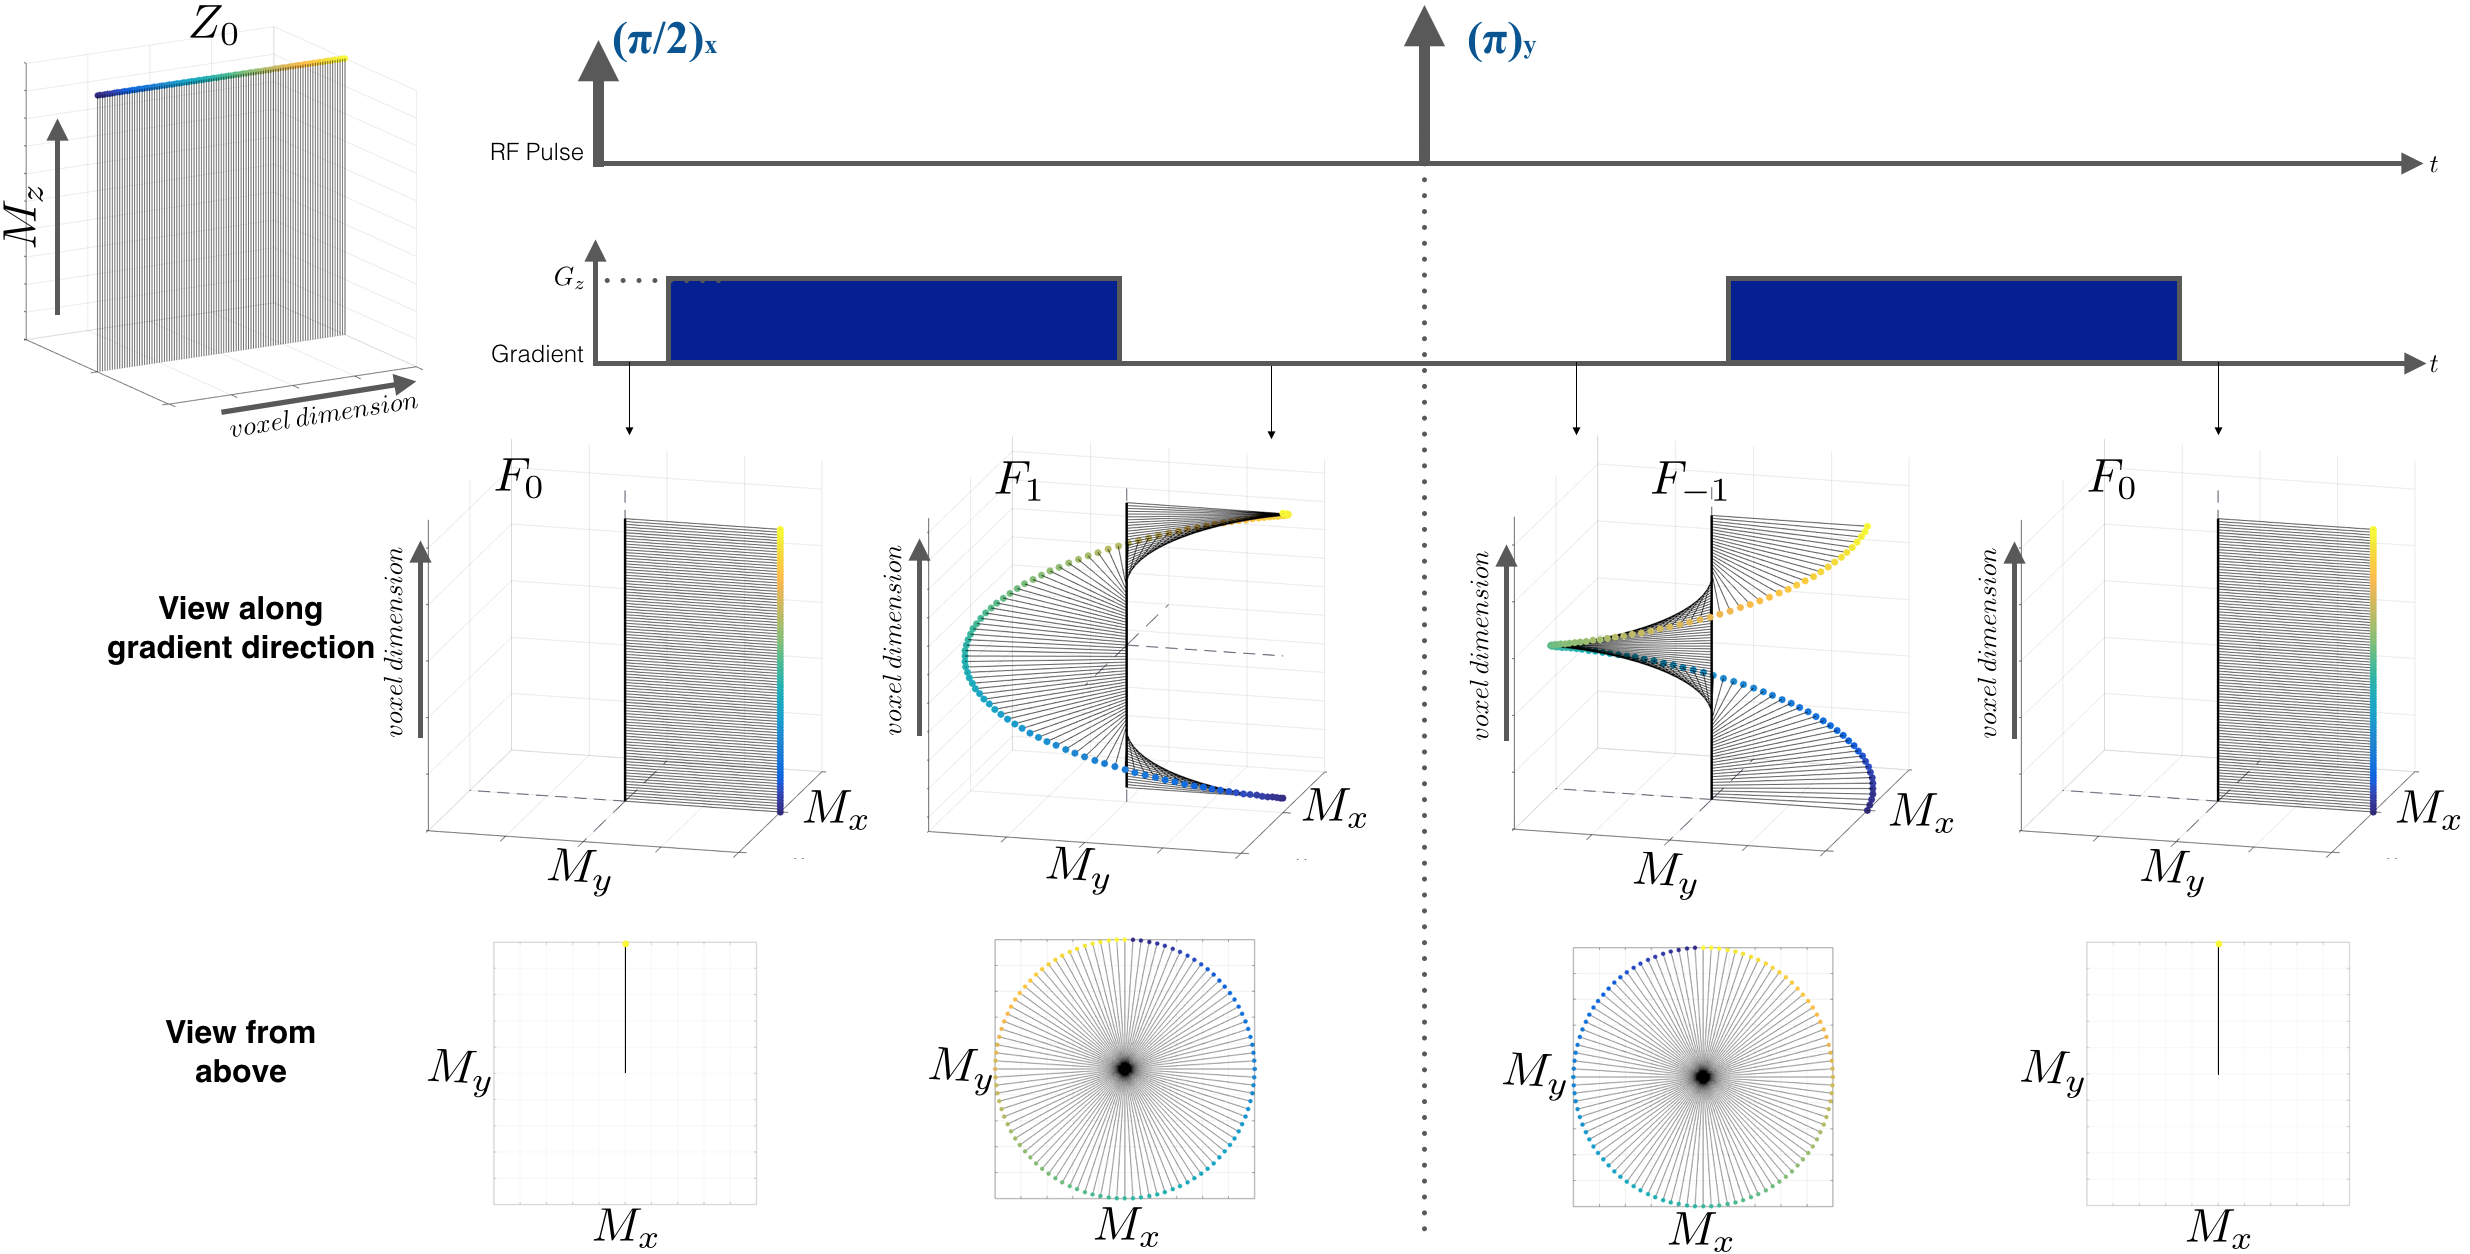
\includegraphics[angle=90,width=0.6\textwidth, keepaspectratio]{images/mrf/spinechoinepg}
    \caption{Pictorial representation of the formation of a spin echo.
    The first RF pulse flips the distribution of isochromats into the $\bm{F_0}$ configuration.
    The application of the gradient dephases the spins until the $\bm{F_1}$ configuration is formed.
    The application of the second RF pulse of flip angle $180^o$ yields the $\bm{F_{-1}}$ configuration.
    The application of the second gradient rephases the spins until they reach the coherent state $\bm{F_0}$ and an echo is formed.}
    \label{fig:spinechoinepg}
\end{figure}

The formation of the $F_{-k}$ states is best explained through an example where an RF pulse of $\alpha = \pi$ and $\phi = \pi/2$ (rotation about the y-axis) is applied on an $\bm{F_1}$ configuration.
Introducing these values in equation \ref{eq:woessner} yields:

\begin{equation}
\begin{split}
    F_{1}^+  &= - F_{-1}^- = 0 \\
    F_{-1}^+ &= - F_{1}^-  \\
    Z_{1}^+  &= - Z_{1}^- = 0
\end{split}
\end{equation}
where the $F_{-1}^-$ and $Z_{1}^-$ were set to $0$ because they were non-existent prior to the RF pulse application.
This shows that the $F_{-1}$ configuration is now formed as a consequence of applying an $180^o$ refocusing pulse.
This is the mechanism through which spin echoes are formed and a pictorial example of this happening is shown in Figure~\ref{fig:spinechoinepg}.

\hfill

The formation of the $Z_{k}$ states is best explained through an example where the RF pulse has a flip angle $\neq \pi$.
Let there be an RF pulse of flip angle $\alpha = \pi/4$ and phase angle $\phi = 0$ applied on an $\bm{F_1}$ configuration.
Introducing these values in equation \ref{eq:woessner} yields:

\begin{equation}
\begin{split}
    F_{1}^+  &= F_{1}^- cos^2(\alpha/2) \approx 0.853 F_{1}^- \\
    F_{-1}^+ &= F_{1}^- sin^2(\alpha/2) \approx 0.147 F_{1}^-   \\
    Z_{1}^+  &= - i/2 F_{1}^- sin(\alpha)  \approx - 0.353 \, i \, F_{1}^-
\end{split}
\end{equation}
which shows that the application of the RF pulse lead to a partitioning of the isochromat ensemble into three configuration states: $\bm{F_1}$, $\bm{F_{-1}}$ and $\bm{Z_1}$ of different coefficients.
Figure~\ref{fig:RFPulseinEPG} shows a pictorial representation of the effect of applying the $(\pi/4)_x$ RF pulse on a dephased $\bm{F_1}$ configuration.

\begin{figure}[ht]
    \centering
    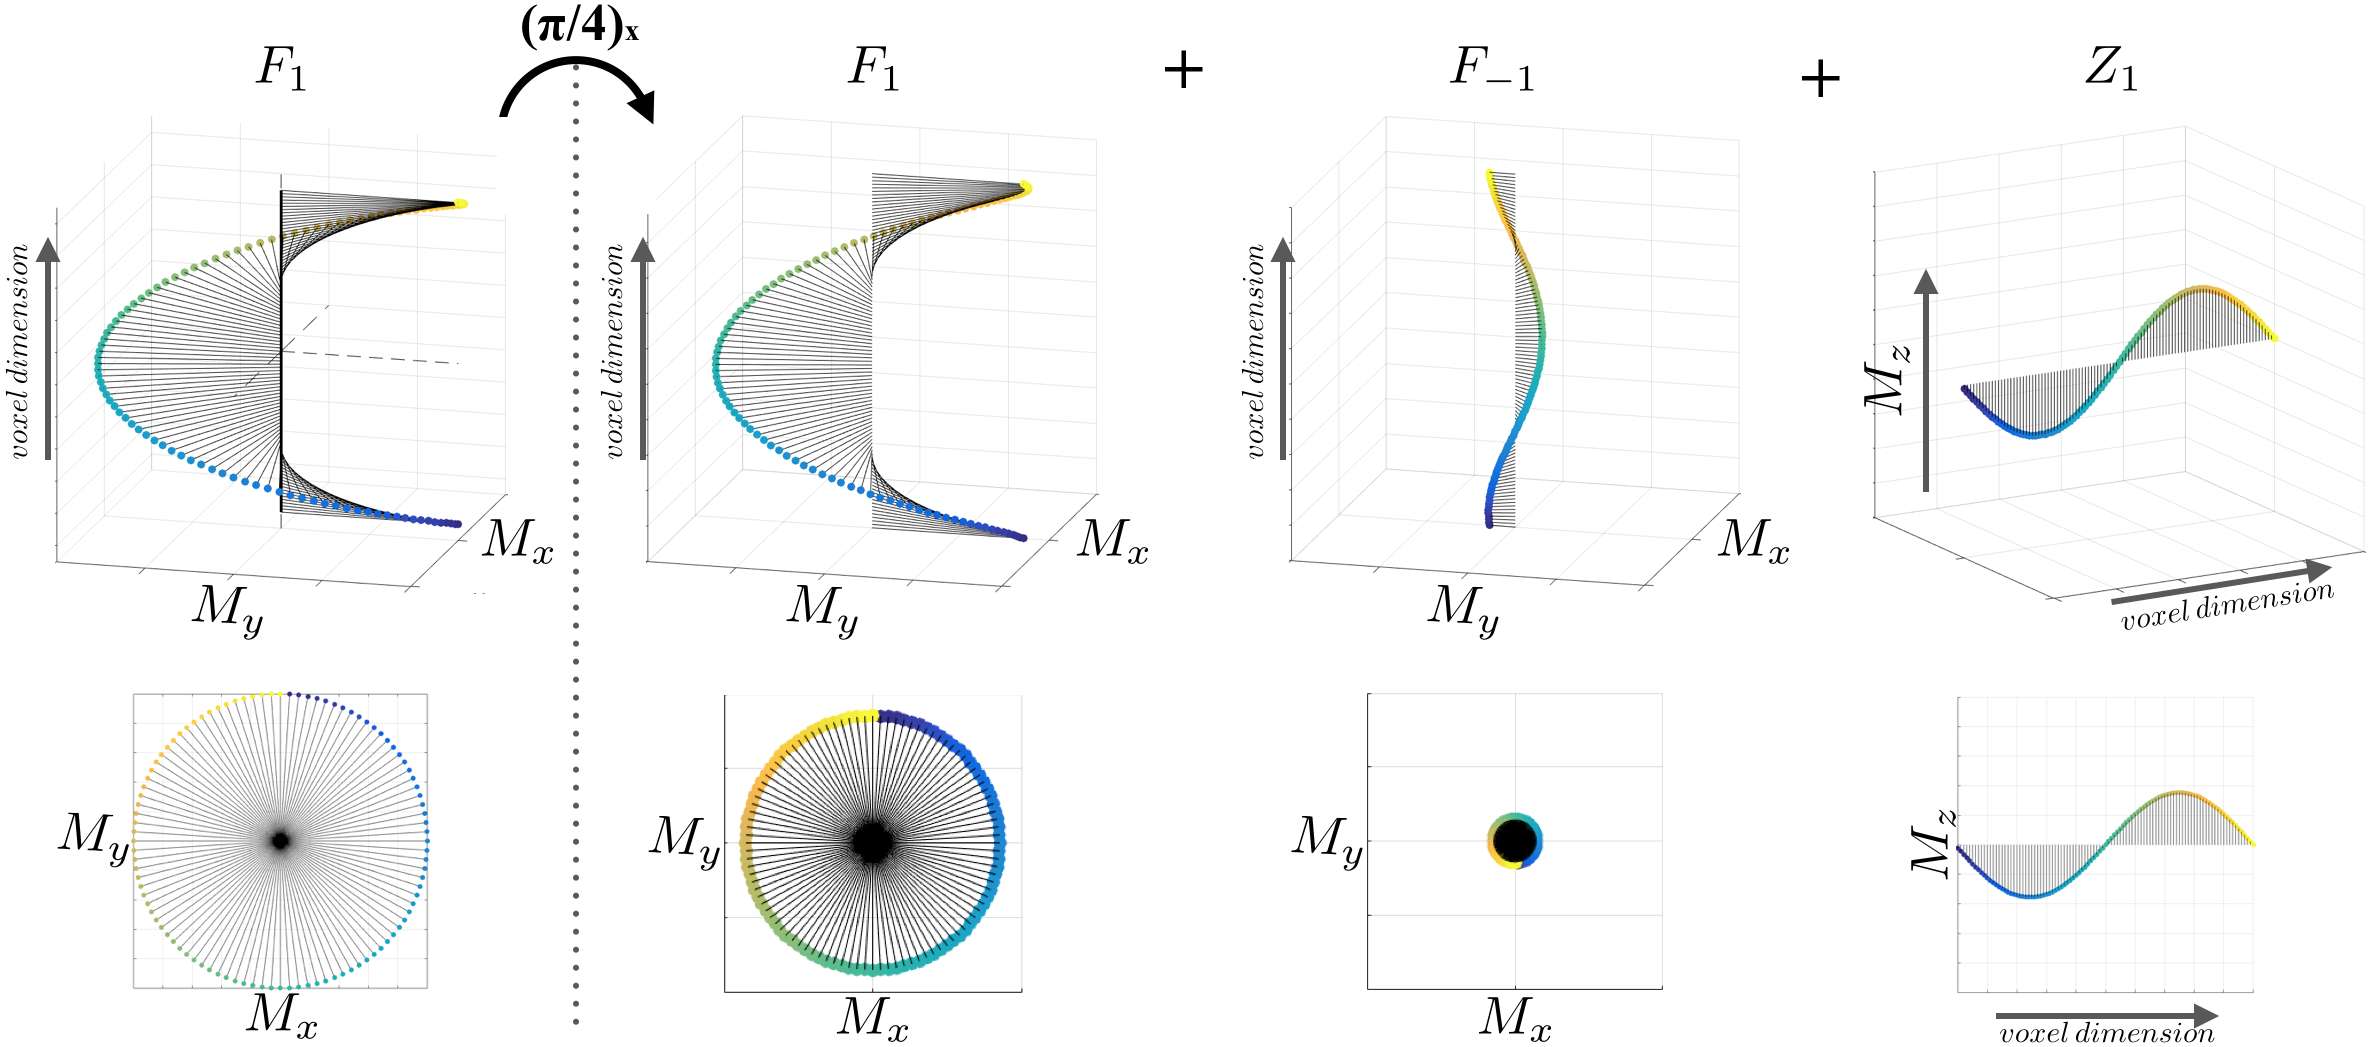
\includegraphics[angle=0,width=1\textwidth, keepaspectratio]{images/mrf/RFPulseinEPG}
    \caption{Pictorial representation of the formation of configuration states as a result of applying an RF pulse on a fully dephased $\bm{F_1}$ state.
    In this example we are showing the effect of an instantaneous RF pulse of flip angle $\alpha = \pi/4$ and phase angle $\phi = 0$ which `mixes' the populations into configuration states of the same 
    }
    \label{fig:RFPulseinEPG}
\end{figure}

\hfill

% % % % % % % % % % % % % % % % % % % % 
\textbf{Relaxation effects} 

The effects of relaxation towards thermal equilibrium can also be described in the \ac{epg} framework.
For the transverse states $T_2$ relaxation occurs: $F_k' = E_2 F_k$, while for the longitudinal states $T_1$ relaxation occurs: $Z_k' = E_1 Z_k$ (for $k \neq 0$)
%, $Z_k$ states are attenuated) 
and $Z_k' = E_1 Z_k + M_0(1 - E_1)$ (for $k = 0$).
%, $Z_k$ states experience recovery).
Here, $E_1 = e^{-\tau/T_1}$ and $E_2 = e^{-\tau/T_2}$ for a given time $\tau$.
In matrix form, this becomes \cite{Hennig1991}:

\begin{equation}\label{eq:woessnerFn}
    \begin{bmatrix}
        F_k      \\
        F_{-k} \\
        Z_k
    \end{bmatrix}' = 
    \underbrace{
    \underbrace{\begin{bmatrix}
        E_2 & 0 & 0 \\
        0 & E_2 & 0 \\
        0 & 0 & E_1 
    \end{bmatrix}
    \begin{bmatrix}
        F_k      \\
        F_{-k} \\
        Z_k
    \end{bmatrix}}_\text{for k $\neq$ 0}
    +
    \begin{bmatrix}
        0 \\
        0 \\
        M_0 (1 - E_1)
    \end{bmatrix}}_\text{for k = 0}
\end{equation}

\hfill

\large \textbf{Extended Phase Graph Algorithms} \normalsize

The \ac{epg} algorithm consists of a set of rules to be applied in order to simulate signals coming from a wide variety of MR sequences.
I start by describing the key data structures involved in the algorithm and then move on to explaining how RF pulses, dephasing gradients and relaxation phenomena are introduced in this framework.

\hfill

\textbf{EPG Data Structures}

In the \ac{epg} algorithm the set of all possible confugration states at any given time point is stored in a matrix called the `state matrix':
\begin{equation}
    \Omega = 
    \begin{bmatrix}
    F_0 & F_1 & F_2 & \dots \\
    F_0^* & F_{-1} & F_{-2} & \dots \\
    Z_0 & Z_1 & Z_2 & \dots 
    \end{bmatrix}
\end{equation}
where $\bm{F_0}$ occurs twice for completion.

\hfill

This matrix contains the three possible basis states $\bm{F_k}$, $\bm{F_{-k}}$ and $\bm{Z_k}$ in increasing dephasing order $\bm{k}$.
Although this matrix can be considered infinite in one dimension as there are infinitely many configurations, all MR experiments are finite thus limiting the matrix size to reasonable dimensions.
In fact, for the sequence I am modelling, where both the repetition time and the amount of dephasing in each period is constant, the number of branches is equal to the number of RF pulses.
Thus, the state matrix $\Omega$ is a $3 \times N_{pulses}$ complex matrix that stores the coefficients for each basis set.

\hfill

In order to store all the possible configuration states for all time points $t$ in the multi-pulse sequence, two other matrices are used, called the `evolution matrices':

\begin{equation}
    \Xi_F = 
    \begin{bmatrix}
    \vdots & \vdots & \vdots & \vdots & \dots \\
    F_2(t_0) & F_2(t_1) & F_2(t_2) & F_2(t_3) & \dots \\
    F_1(t_0) & F_1(t_1) & F_1(t_2) & F_1(t_3) & \dots \\
    F_0(t_0) & F_0(t_1) & F_0(t_2) & F_0(t_3) & \dots \\
    F_{-1}(t_0) & F_{-1}(t_1) & F_{-1}(t_2) & F_{-1}(t_3) & \dots \\
    F_{-2}(t_0) & F_{-2}(t_1) & F_{-2}(t_2) & F_{-2}(t_3) & \dots \\
    \vdots & \vdots & \vdots & \vdots & \dots 
    \end{bmatrix}
\end{equation}

and

\begin{equation}
    \Xi_Z = 
    \begin{bmatrix}
    \vdots & \vdots & \vdots & \vdots & \dots \\
    Z_2(t_0) & Z_2(t_1) & Z_2(t_2) & Z_2(t_3) & \dots \\
    Z_1(t_0) & Z_1(t_1) & Z_1(t_2) & Z_1(t_3) & \dots \\
    Z_0(t_0) & Z_0(t_1) & Z_0(t_2) & Z_0(t_3) & \dots 
    \end{bmatrix}
\end{equation}

\hfill

The evolution matrices store the state matrices, as columns, for each time point of interest.
These matrices can, again, be of infinite size, as there are infinite configurations and the time domain can be infinitely sampled.
However, for my application where both the repetition time and the amount of dephasing in each period is constant, the $\Xi_F$ evolution matrix is a $2N_{pulses}-1 \times N_{pulses}$ complex valued matrix, while the $\Xi_Z$ evolution matrix is an $N_{pulses} \times N_{pulses}$ complex valued matrix.
This is because I am only interested in the values of the coefficients at echo time in each $T_R$ block.

\hfill

\textbf{Applying an RF pulse}

RF pulses are modelled as instantaneous by applying the $T_{\phi}(\alpha)$ operator (see equation \ref{eq:woessnerFn2}) on the pre-RF pulse state matrix.
For example, for an RF pulse of flip angle $\alpha = \pi/2$ and phase angle $\phi = 0$ applied on the initial $\Omega (t < 0) = [0, 0, 1]^T$, we write:
\begin{equation}
    \Omega (t = 0) = T_0(\pi/2) \Omega (t < 0) = 
    \begin{bmatrix} 
        1 \\
        1 \\
        0
    \end{bmatrix}
\end{equation}

\hfill

\textbf{Dephasing due to gradient}

As stated before, dephasing causes a shift of configuration states.
Thus, it can be represented by a shift operator, $S$, which performs $F_k \rightarrow F_{k+1}$ and leaves the longitudinal state unchanged $Z_k \rightarrow Z_k$. 
For example, if after the application of the $\pi/2$ RF pulse a gradient is applied until the end of the repetition period, the state matrix becomes:
\begin{equation}
    \Omega (t = T_R) = S \, \, \Omega (t = 0) = 
    \begin{bmatrix} 
        0 & 1\\
        0 & 0\\
        0 & 0
    \end{bmatrix}
\end{equation}
where $S$ is the shift operator which performs $F_n \rightarrow F_{n+1}$ and leaves the longitudinal state unchanged $Z_n \rightarrow Z_n$. 
Note that the state matrix contains all possible states, which means that for this example $F_{-1} = 0$ was shifted to $F_0^*$.

\hfill

\textbf{Relaxation}

Relaxation phenomena is treated as explained previously (see equation \ref{eq:woessnerFn}):
all transverse states in the state matrix experience $T_2$ decay, all longitudinal states with $k \neq 0$ in the state matrix experience $T_1$ relaxation and longitudinal states with $k = 0$ also experience $T_1$ recovery.

\hfill

\large \textbf{Dictionary} \normalsize

In order to create a dictionary of signals for a multi-pulse \ac{fisp} sequence, the \ac{epg} algorithm was used.
As with the \ac{bssfp} case, a signal of N time points is created for each `tissue tuple'
$(T_{1_j}, T_{2_j})$, with $j \in [1, M]$, where $M$ is the total number of tuples.
For the \ac{fisp} dictionary, off-resonance frequencies were not included.
The sequence used is found in Figure~\ref{fig:sequenceFISP}, where the echo times were kept constant for every repetition block, and the unbalanced gradients achieved the same amount of dephasing in each $T_R$ block.

\hfill

To generate the signal for a given tissue type, the multi-pulse MRF-\ac{fisp} sequence was divided into $N+1$ blocks (including the inversion pulse), each of which corresponding to the application of a different RF pulse.
The signal corresponds to the $F_0$ states at echo time for each $T_R$ block.
This process was then repeated for every tissue tuple and a dictionary of $M \times N$ complex values was created.
Pseudocode for the algorithm can be found in Appendix~\ref{appendixlabel2}.

\hfill

% Prior to the second RF pulse, due to the presence of the idealised dephasing gradient,
% the spins will accrue different phases, ranging from $-\pi$ in one corner of the voxel, to $+\pi$ in the opposite corner.
% This state in which the transverse magnetisation is now found is called $F_1$ \cite{Hennig1988} \cite{Scheffler1999} and can be conceptually described as an evenly distributed collection of magnetisation vectors over the transverse plane (see Figure~\ref{fig:F1state}). 

% For a single-voxel multi-pulse \ac{fisp} experiment let us now consider that the gradient's moment induces the same amount of dephasing across this voxel during a fixed time period $\Delta t$ at the end of each repetition period.
% For an idealised gradient and an idealised voxel with uniform density of magnetisation,
% the amount of dephasing is defined by the interval $[-\pi, \pi]$.

% \hfill

% \begin{figure}[ht]
%     \centering
%     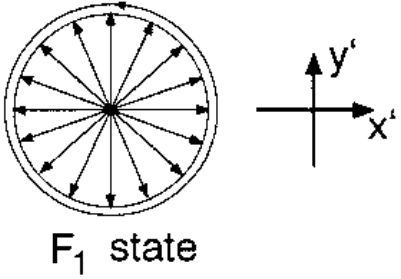
\includegraphics[angle=0,width=0.4\textwidth, keepaspectratio]{images/mrf/F1state}
%     \caption{The $F_1$ state is a magnetisation substate which describes a uniform distribution of magnetisation vectors over the transverse plane, with phases ranging from $-\pi$ to $+\pi$. Figure adapted from \cite{Scheffler1999}.}
%     \label{fig:F1state}
% \end{figure}

% \hfill

% The EPG algorithm \cite{Hennig1988} \cite{Hennig1991} \cite{Weigel2015} is a tool used to simulate signals obtained from a wide variety of MRI pulse sequences \cite{Malik2017}.
% % EPG has been used for a variety of applications such as:
% % characterization of RF spoiling in gradient echo sequences (4,5), 
% % analysis of echo amplitudes in turbo spin echo (TSE) sequences (6–9), 
% % diffusion effects (12), and 
% % characterizing signal evolution in sequences used for relaxometry (13–16).
% Similar to the Bloch equations approach, EPG characterizes a given sequence through the effects of RF pulses, relaxation constants, and dephasing due to gradients or inhomogeneities in the main magnetic field.
% % However, unlike the previous approach, EPG describes a spin system as a discrete set of phase states (or, `configuration states') \cite{Hennig1988}.
% % These states appear as a consequence of 
% To model the behaviour of a spin ensemble with known relaxation times and proton density values in a single-voxel MRF-\ac{fisp} sequence, the following assumptions were made:



% \textbf{Extended Phase Graph Formalism} 

% In the following section three key concepts that form the basis for understanding EPG are presented.
% Next, these concepts are brought together to form the EPG framework.

% \hfill

% % To understand how EPG works, we will first define the total magnetisation $M$ at thermal equilibrium as a normalised column vector $B = [0 \, 0 \, 1]^T$.
% % $B$ contains the coefficients for the $M_x$, $M_y$ and $M_z$ components of the total magnetisation M.
% % At any time point during a multi-pulse experiment, one can calculate the total magnetisation by summing over a collection of spins which are described by their corresponding x,y,z components.
% % However, to be accurate, this requires a large spin ensemble.

% % \hfill

% % In the EPG formalism the matrix $B$ is expanded to describe \textit{substates}.
% % These substates are defined as collection of spins with different $M_x$, $M_y$ and $M_z$ components and are characterised by the net magnetisation of the substate, and the space-dependent phase of the transverse magnetisation of the spin ensemble \cite{Hennig1988}.
% % In this framework, the signal intensity at any given time point during the sequence can be calculated by knowing the partitioning of the total magnetisation between the substates, and the net magnetisation in each substate.

% % \hfill

% \textbf{The effect of gradients on a spin ensemble} 

% For a single-voxel multi-pulse \ac{fisp} experiment let us now consider that the gradient's moment induces the same amount of dephasing across this voxel during a fixed time period $\Delta t$ at the end of each repetition period.
% For an idealised gradient and an idealised voxel with uniform density of magnetisation,
% the amount of dephasing is defined by the interval $[-\pi, \pi]$.

% \hfill 

% Let us consider that the first RF pulse is an ideal $90^o$ excitation pulse which flips the total magnetisation in the transverse plane.
% Prior to the second RF pulse, due to the presence of the idealised dephasing gradient,
% the spins will accrue different phases, ranging from $-\pi$ in one corner of the voxel, to $+\pi$ in the opposite corner.
% This state in which the transverse magnetisation is now found is called $F_1$ \cite{Hennig1988} \cite{Scheffler1999} and can be conceptually described as an evenly distributed collection of magnetisation vectors over the transverse plane (see Figure~\ref{fig:F1state}). 

% \begin{figure}[ht]
%     \centering
%     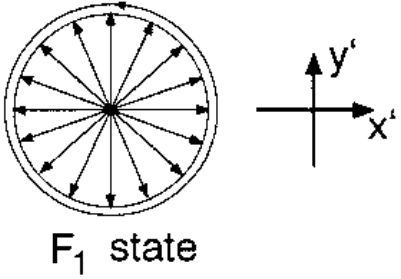
\includegraphics[angle=0,width=0.4\textwidth, keepaspectratio]{images/mrf/F1state}
%     \caption{The $F_1$ state is a magnetisation substate which describes a uniform distribution of magnetisation vectors over the transverse plane, with phases ranging from $-\pi$ to $+\pi$. Figure adapted from \cite{Scheffler1999}.}
%     \label{fig:F1state}
% \end{figure}

% \hfill

% The application of a second RF pulse will interfere with this state.
% For an arbitrary flip angle $\alpha$ and phase angle $\phi = 0$, the $F_1$ `disk' will be rotated around the RF pulse's axis of rotation.
% The newly formed transverse magnetisation can be described as two dephased states: $F^+_1$ and $F^+_{-1}$, while the longitudinal magnetisation is now known as $Z^+_1$.
% The superscript `+' denotes `immediately after the RF pulse'.
% In the EPG formalism, other states exist and they are denoted as $F_n$, depending on the amount of dephasing experienced.
% This can be seen in Figure~\ref{fig:EPGeffectofgrad}, where the $2^{nd}$ gradient pulse further dephased the $F_1$ state.
% Due to being an idealised gradient and an idealised voxel with uniform density of magnetisation, the amount of dephasing is again defined by the interval $[-\pi, \pi]$.
% This causes the spins to have now accrued phases ranging from $-2 \pi$ to $+2 \pi$.
% The presence of the gradient will therefore `transform' the $F_1^+$ state into a new state we call $F_2$.
% On the other hand, $Z^+_1$ was formed because the RF pulse `flipped' the transverse components of some of the pre-RF pulse magnetisation vectors into the longitudinal plane.
% The formation of the $F_1^+$, $F_{-1}^+$ and $Z_1^+$ states is better understood through the Woessner decomposition \cite{Woessner1961}.

% \begin{figure}[ht]
%     \centering
%     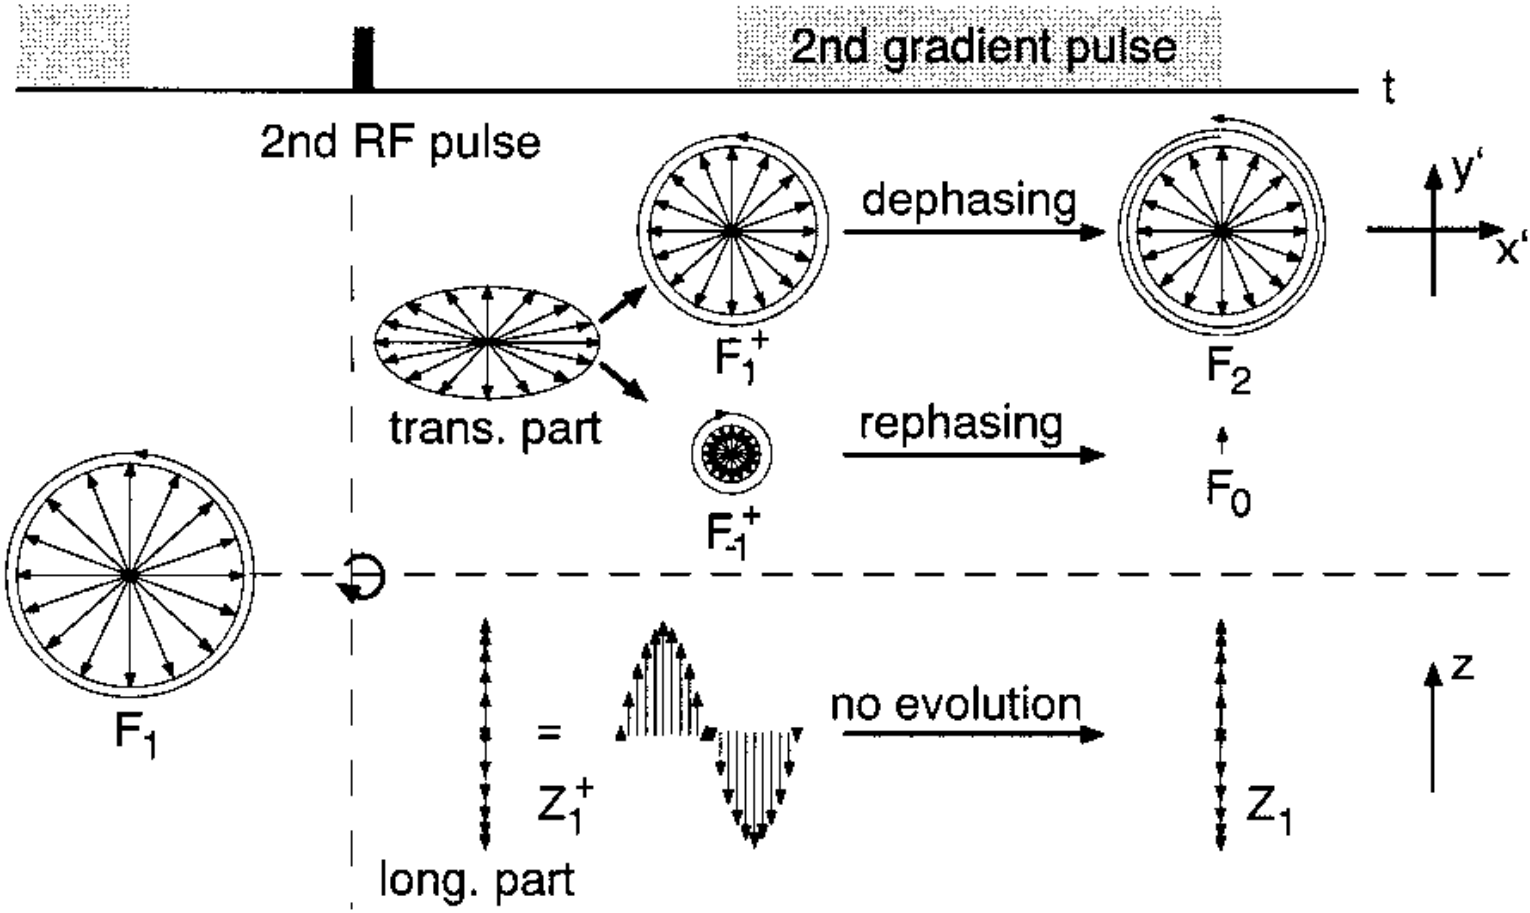
\includegraphics[angle=0,width=0.8\textwidth, keepaspectratio]{images/mrf/EPGeffectofgrad}
%     \caption{A second RF pulse will `split' the previous $F_1$ configuration into two separate transverse state configurations $F_1^+$ and $F_{-1}^+$, and a longitudinal state $Z_1^+$; this process is best described with the \textit{Woessner decomposition}. During the application of the dephasing gradient, the longitudinal state remains unaffected, while the transverse states are further dephased $F_1^+ \rightarrow F_2$, and rephased $F_{-1}^+ \rightarrow F_0$, respectively. Figure adapted from \cite{Scheffler1999}.}
%     \label{fig:EPGeffectofgrad}
% \end{figure}

% \hfill

% \textbf{Woessner decomposition.} The Woessner decomposition describes the behaviour of a complex magnetisation vector $F = M_x + i M_y$ subject to an RF pulse of arbitrary flip angle $\alpha$ and phase angle $\phi$.
% As stated before, the effect of an RF pulse can be written as a rotation matrix, which, when applied to the complex magnetisation vector yields \cite{Haacke1999} \cite{Scheffler1999}:

% \begin{equation}\label{eq:woessner}
% \begin{split}
%     F^+ &= F^- cos^2(\alpha/2) + e^{2i\phi} (F^-)^* sin^2(\alpha/2)  - i e^{i \phi} M_z^- sin(\alpha)  \\
%     M_z^+ &= - i/2 e^{-i \phi} F^- sin(\alpha) + i/2 e^{-i \phi} (F^-)^* sin(\alpha) + M_z^- cos(\alpha) 
% \end{split}
% \end{equation}
% where the superscript \textbf{+} represents immediately `after the RF pulse' and the superscript \textbf{-} represents immediately `before the RF pulse'.

% \hfill

% To make the transition to fully dephased transverse states $F_n$ and longitudinal states $Z_n$, we need to take into account the fact that an $F_n$ state represents a collection of dephased spins at different spatial positions within the idealised voxel.
% For a one-dimensional voxel, the phase of a spin at position $x$ induced by n identical gradient lobes evolves with $e^{i \, n \, \, \gamma G_x x \, \Delta t }$, where $G_x$ is the amplitude of the gradient and $\Delta t$ is its duration.
% For all positions r in the voxel, the dephased transversal state can be written as a sum over all positions: $ F_n \int_r \, dr \, e^{i \, n \, \, \gamma G r \, \Delta t }$, where the amplitude of the complex number $F_n$ represents the magnitude of this state's population.
% Similarly, the longitudinal state can be described as $ Z_n \int_r \, dr \, e^{i \, n \, \, \gamma G r \, \Delta t }$.

% \hfill

% \textbf{RF Pulse. } Introducing the complex dephased states in equations \ref{eq:woessner} and transforming into matrix representation, we can write:

% \begin{equation}\label{eq:woessnerFn1}
%     \begin{bmatrix}
%         F_n      \\
%         F_{-n}^* \\
%         Z_n
%     \end{bmatrix}^+ = 
%     T_{\phi}(\alpha)
%     \begin{bmatrix}
%         F_n      \\
%         F_{-n}^* \\
%         Z_n
%     \end{bmatrix}^- 
% \end{equation}
% where
% \begin{equation}\label{eq:woessnerFn2}
%     T_{\phi}(\alpha) = 
%     \begin{bmatrix}
%         cos^2(\alpha/2) & e^{2i\phi} sin^2(\alpha/2) & - i e^{i \phi} sin(\alpha) \\
%         e^{-2i\phi} sin^2(\alpha/2) & cos^2(\alpha/2) & i e^{-i \phi} sin(\alpha) \\
%         - i/2 e^{-i \phi} sin(\alpha) & i/2 e^{i \phi} sin(\alpha) & cos \alpha
%     \end{bmatrix}
% \end{equation}

% and the $F^*_{-n}$ state represents the complex conjugate of the $F_n$ state.

% \hfill

% Equations \ref{eq:woessnerFn1} and \ref{eq:woessnerFn2} show that, given an ensemble of spins, an RF pulse with flip angle $\alpha$ and phase angle $\phi$ will redistribute the population into different states.
% For example, different amounts of the pre-RF pulse $F^-_n$ state can now be found in both the post-RF pulse transverse state $F^+_n$ and the longitudinal state $Z_n$.
% The population represented by $F^*_{-n}$ state can be interpreted as an isochromat population whose phase was instantaneously inverted by the RF pulse, and which can be rephased later.

% % % % % % % % % % % % % % % % % % % % % % % % % % % % % % % % % % % % % % % % % % % % % % % % % % % % % % % % % % % % % % % % % % % % % % % % % % % % % % % % % % % % % % % % % % % % % % % % % % % % % % % % % % % % % % % % % % % % % % % % % % % % % % % % % % % % % % % % % % % % % % % % 
\subsection{Image Space Simulation}
\label{method:imagespace}

The second step in the simulation framework consists of the image space simulation of an IR-bSSFP MRF experiment.
This involves four components (digital object, acquisition sequence, reconstruction and motion) which are covered next.

% % % % % % % % % % % % 
\subsubsection{Digital Object}

For the simulations involved a digital phantom of $80mm$ in diameter, consisting of 12 circular structures of $5mm$ in diameter was created.
The resolution of this phantom is of $1mm$.
%, and the spin density was chosen such that there is a single spin isochromat present at each spatial location $\vec{r}$ in the phantom.
The distribution of $T_1$ and $T_2$ relaxation times is shown in Figure~\ref{fig:inputObject}, while the spin density is set to $\rho(\vec{r}) = 1$ everywhere inside the phantom, except for the space between the `tubes' and the circular phantom.
The range of values chosen for the relaxation times are also summarised in Appendix~\ref{appendixlabelPhantom}.

\begin{figure}[ht]
    \centering
    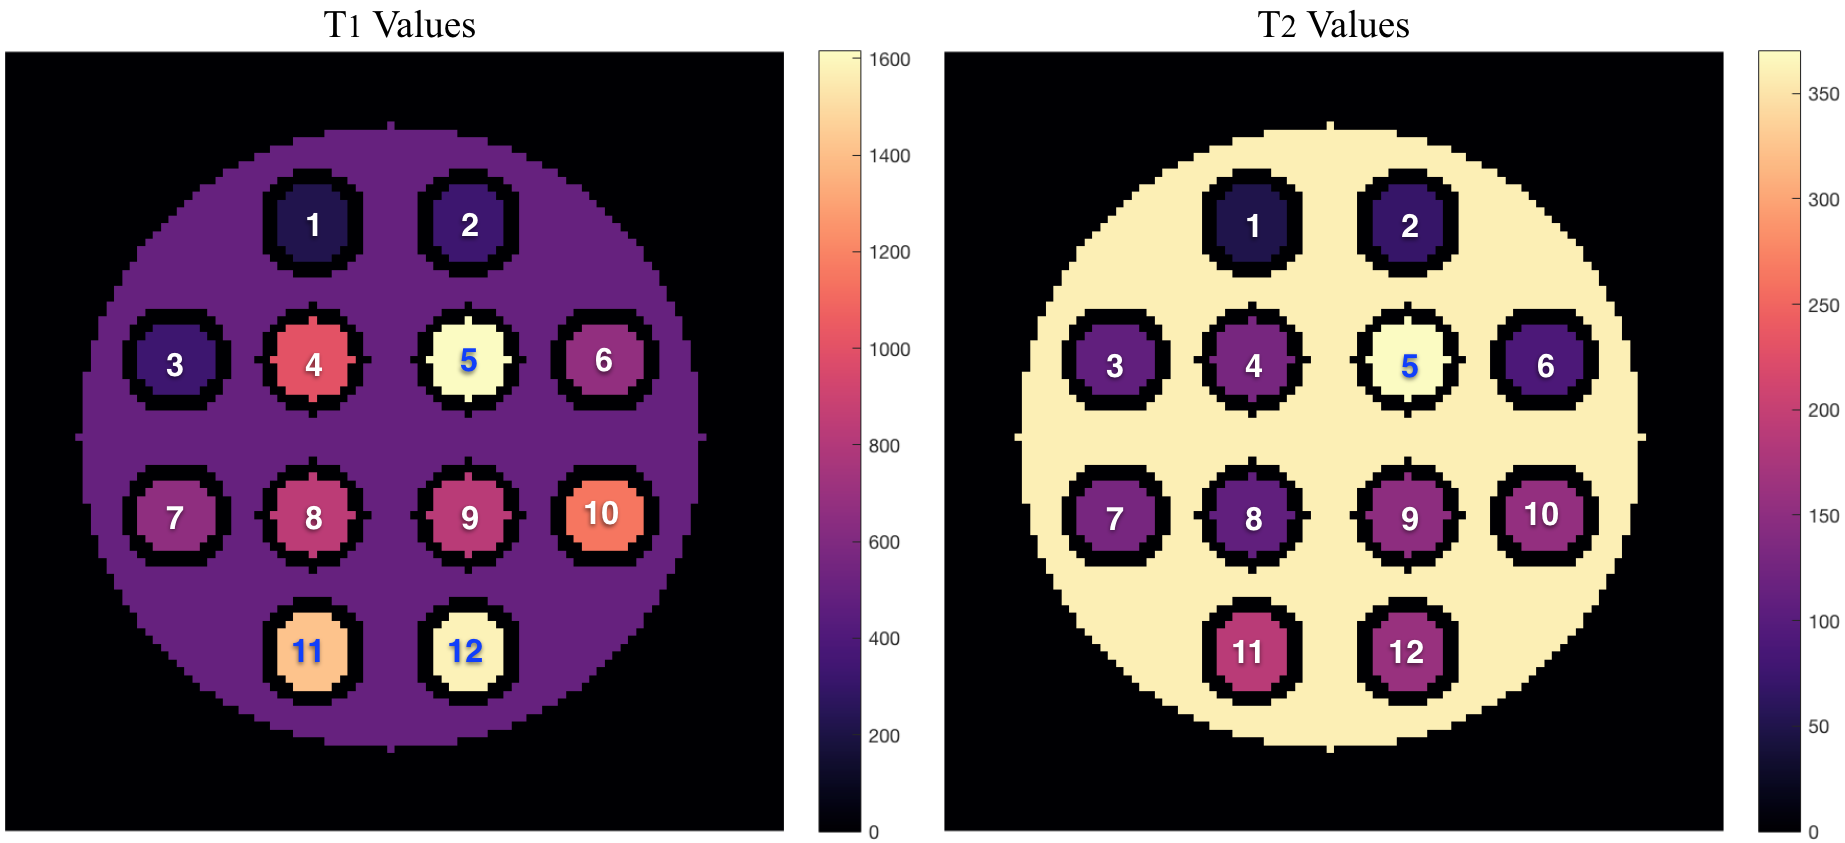
\includegraphics[angle=0,width=1\textwidth, keepaspectratio]{images/mrf/inputObject}
    \caption{The input object is a circular phantom of $80mm$ in diameter, consisting of 12 circular structures of $5mm$ in diameter. Each `tube' (shown here with indices ranging from 1 to 12) has a different $T_1$ and $T_2$ value. Similarly, the surrounding structure has its own relaxation parameters (index 0). $T_1$ and $T_2$ values are summarised in a table in Appendix~\ref{appendixlabelPhantom}.}
    \label{fig:inputObject}
\end{figure}

\hfill

The choice of digital phantom structure and composition is based on the \textit{Eurospin} 
phantom set, Test Object 5 (TO5), which contains 12 holes for agarose gel sample tubes with different relaxation properties \cite{Ihalainen2004} (see Figure~\ref{fig:realPhantom}).
The values for the relaxation times were chosen from the provided $T_1$ and $T_2$ Eurospin Appendix table and correspond to 12 of the 18 available tubes.
Moreover, this type of phantom was used in previous MRF studies such as those presented in \cite{Doneva2016} and \cite{Sommer2017}.

\begin{figure}[ht]
    \centering
    
\includegraphics[angle=0,width=0.4\textwidth, keepaspectratio]{images/mrf/realPhantom}
    \caption{The figure shows the Eurospin Test Object 5 (TO5) real phantom used for MRI quality control.
    More specifically, the TO5 of the Eurospin phantom set is used for measuring $T_1$ and $T_2$ precision and accuracy.
    The object consists of a homogeneous cylinder with 12 holes in which sample tubes of different gels with different relaxation properties can be inserted. Image courtesy of \cite{Ihalainen2004}.}
    \label{fig:realPhantom}
\end{figure}

% % % % % % % % % % % % 
\subsubsection{Acquisition}

The sequence used for the image space simulations is based on the initial implementation of the MRF framework by Ma et al. \cite{Ma2013} and is known as an inversion recovery balanced steady state free precession sequence (IR-\ac{bssfp}).
The sequence diagram is shown in Figure~\ref{fig:sequencebSSFP}.
The only difference between the sequence used for the dictionary generation part and the one used for the image acquisition part of the simulations is that the latter one was equipped with a spiral readout of duration $6 ms$.
Moreover, the spiral readout is accompanied by rewinding gradients that take the trajectory back to the centre of k-space and also assure that the zeroth moment of all gradients is zero at the end of a repetition period.

\begin{figure}[ht]
    \centering
    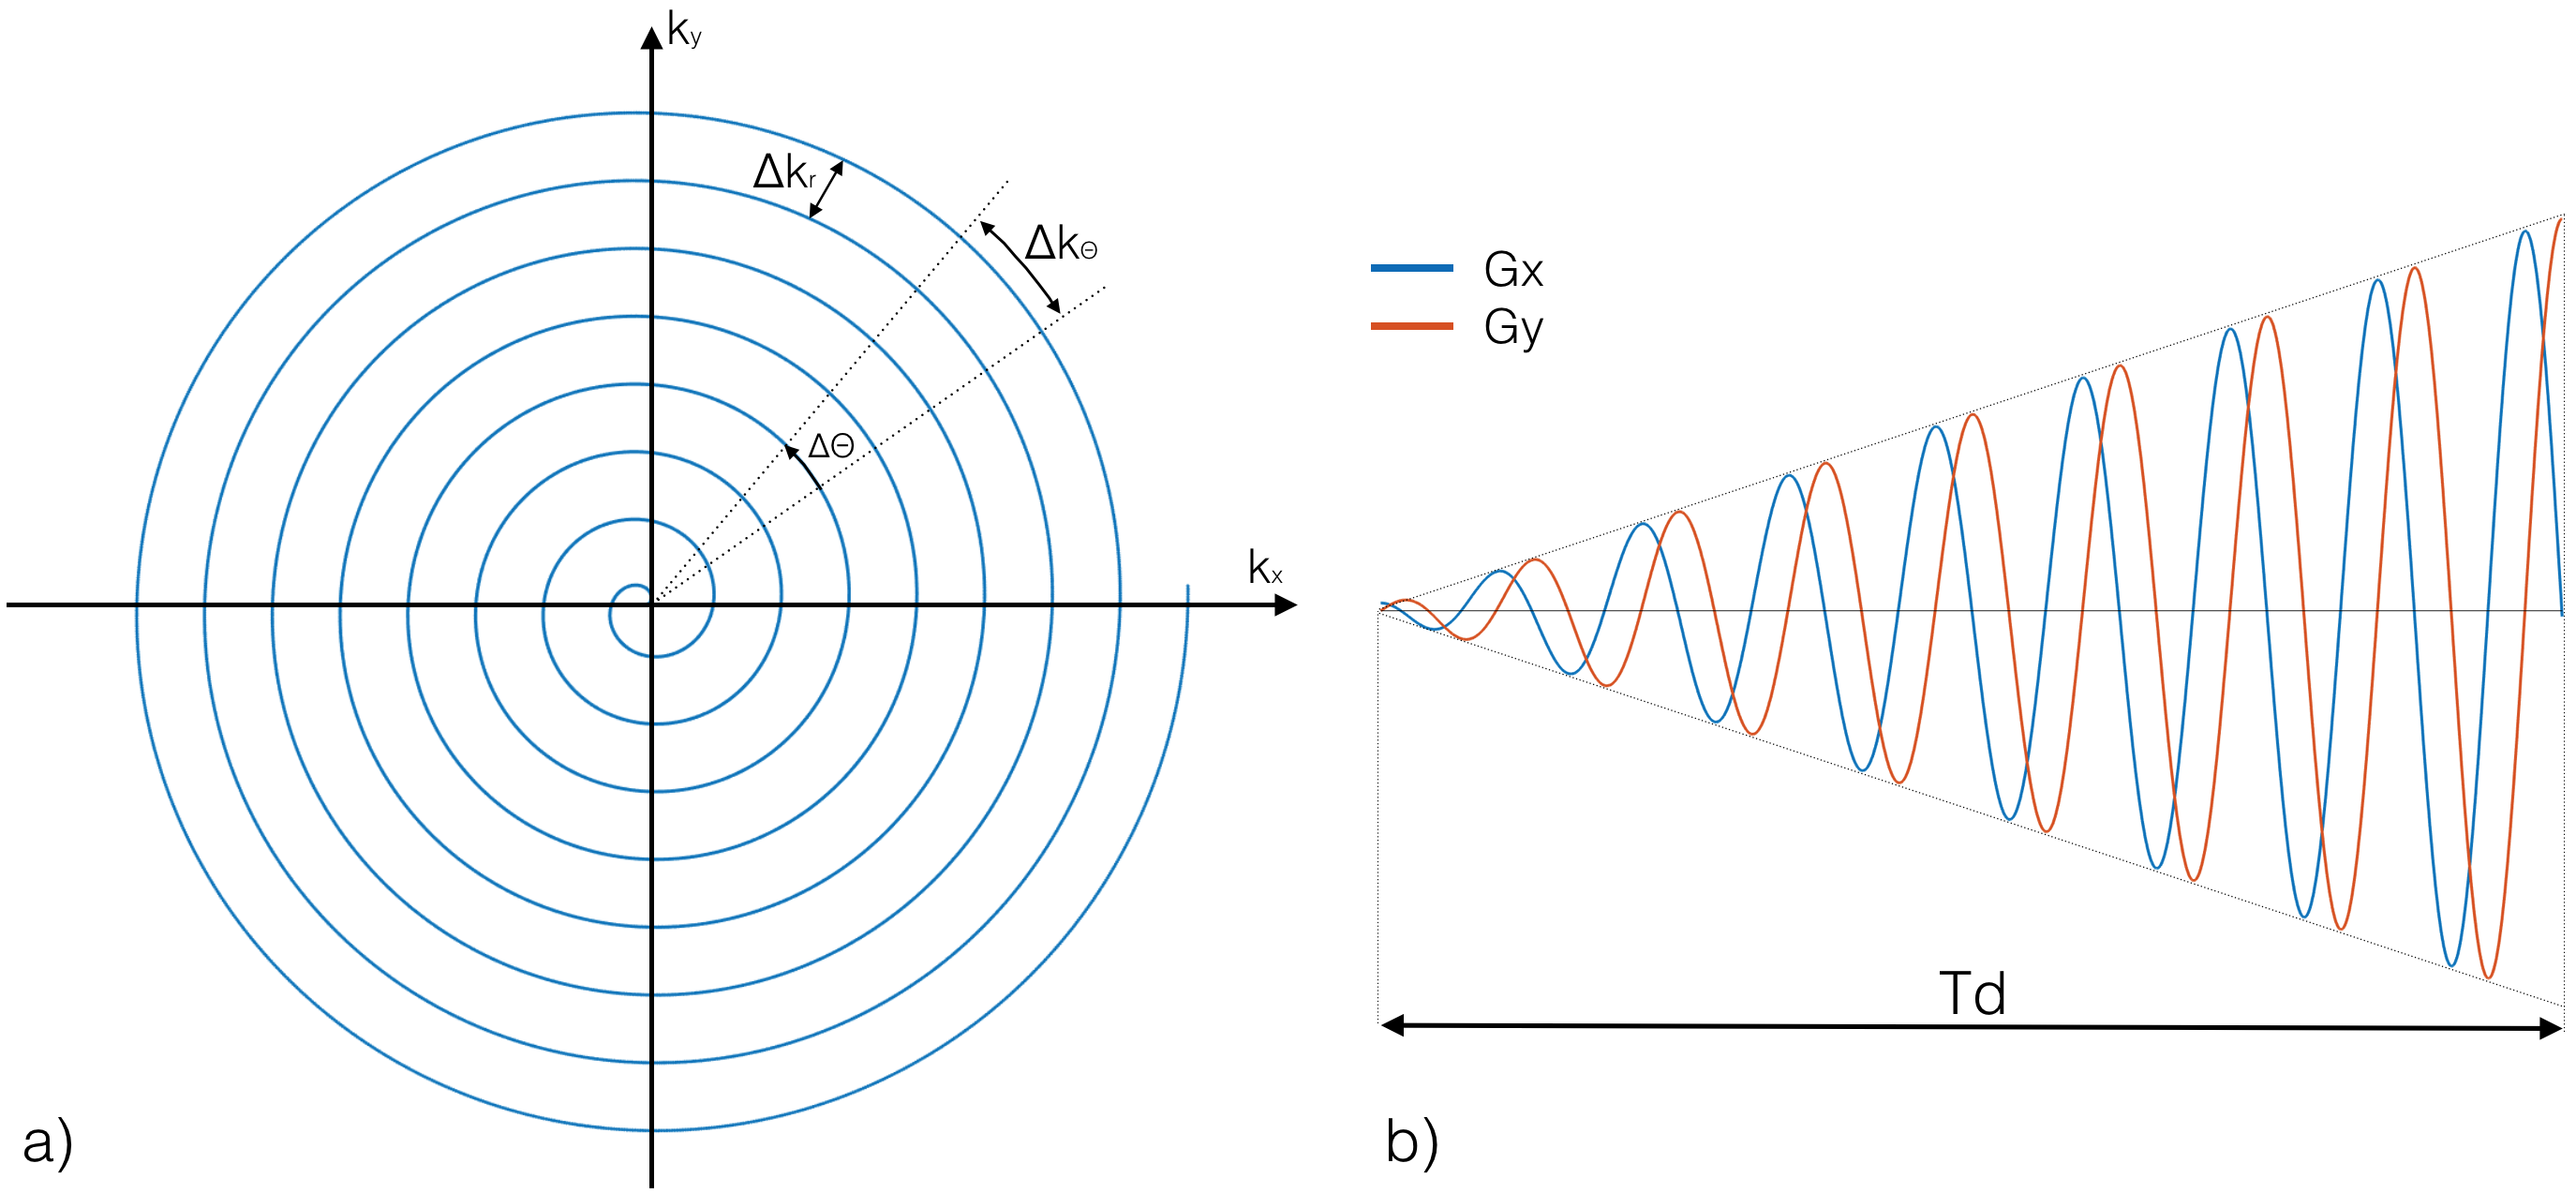
\includegraphics[angle=0,width=1\textwidth, keepaspectratio]{images/mrf/spiralAcquisition}
    \caption{An illustration of the linearly increasing spiral acquisition, showing a) the k-space trajectory and b) the corresponding gradient shape for this trajectory}
    \label{fig:spiralAcquisition}
\end{figure}

\hfill

The spiral readout was constructed in JEMRIS by analytically describing the shape of the k-space trajectory.
While different spiral coverages of k-space exist, for my simulations I chose a linearly increasing sinusoidal form, also known as a constant angular velocity (Archimedean) spiral trajectory first proposed by Ahn et al. \cite{Ahn1986}. 
Mathematically, the k-space trajectory takes the following form:

\begin{equation}\label{eq:kspacespiral}
    \begin{split}
        k_x(t) &= \text{\sout{$\gamma$}} \, \, \alpha_1 t \, \, cos (\alpha_2 t) \\
        k_y(t) &= \text{\sout{$\gamma$}}  \, \, \alpha_1 t  \, \, sin (\alpha_2 t) 
    \end{split}
\end{equation}

where $\alpha_1$ determines the gradient amplitude and $\alpha_2$ determines the angular frequency.
From equation \ref{eq:kspacespiral} and from knowing that $k_x(t) = \text{\sout{$\gamma$}} \, \, \int_0^t G_x(t') dt'$ and $k_y(t) = \text{\sout{$\gamma$}} \, \, \int_0^t G_y(t') dt'$ (see equation \ref{eq:kspace}), the desired time domain gradients can be found:

\begin{equation}
    \begin{split}
        G_x(t) &= \frac{1}{\text{\sout{$\gamma$}}} \frac{d}{dt} \,\, [k_x(t)] = \alpha_1 cos (\alpha_2 t) - \alpha_1 \alpha_2 t sin (\alpha_2 t) \\
        G_y(t) &= \frac{1}{\text{\sout{$\gamma$}}} \frac{d}{dt} \,\, [k_y(t)] = \alpha_1 sin (\alpha_2 t) + \alpha_1 \alpha_2 t cos (\alpha_2 t) 
    \end{split}
\end{equation}

The shape of both the k-space trajectory and the gradient waveforms can be seen in Figure~\ref{fig:spiralAcquisition}, where $t \in [0, T_d]ms$.

\hfill

Constant angular velocity Archimedean spirals have constant step sizes in both radial ($\Delta k_r$) and azimuthal directions ($\Delta k_{\theta}$).
The values for these step sizes can be found by considering the sampling requirements imposed by the Nyquist criterion.
For this, we first need to rewrite the k-space trajectory in polar coordinates:
\begin{equation}
    \begin{split}
        k_r(t) &= \sqrt{k_x^2(t) + k_y^2(t)} = \text{\sout{$\gamma$}} \alpha_1 t \\
        k_{\theta}(t) &= tan^{-1} \Bigg[ \frac{k_y(t)}{k_x(t)} \Bigg] = \alpha_2 t
    \end{split}
\end{equation}

Now, considering constant numbers of sampling points per winding $n_{\theta}$ and radially $n_r$, and knowing that two radial points are exactly $2\pi$ apart, both angular and radial step sizes can be defined:
\begin{equation}\label{eq:deltak1}
    \Delta k_r = \text{\sout{$\gamma$}} \alpha_1 n_{\theta} \Delta t  \, \, \text{  and  } \, \, \Delta k_{\theta} = \alpha_2 \Delta t
\end{equation}
where $\Delta t$ is the sampling rate.
% \Delta k_r = k_r(t) \rvert_{t=t'+2\pi/\alpha_2} + k_r(t) \rvert_{t=t'}
To find the required number of sampling points, we can also write:
\begin{equation}\label{eq:deltak2}
    \Delta k_r = \frac{k_{max}}{n_r} = \frac{1}{2 \Delta r n_r} \leq \frac{1}{L} \, \, \text{  and  } \, \,  \Delta k_{\theta} = k_{max} \Delta \theta = \frac{2 \pi}{2 \Delta r n_{\theta}} \leq \frac{1}{L} 
\end{equation}
where $\Delta r$ is the image resolution.
Therefore, for a fully sampled spiral we choose: $n_r \geq L / 2 \Delta r$ and $n_{\theta} \geq \pi L / \Delta r$.

\hfill

Explicit values for $\alpha_1$ and $\alpha_2$ are found from equations \ref{eq:deltak1} and \ref{eq:deltak2}:
\begin{equation}
    \alpha_1 = \frac{\pi}{\text{\sout{$\gamma$}} n_{\theta} n_r \Delta t \Delta r}  \, \, \text{  and  } \, \, \alpha_2 = \frac{2 \pi}{n_{\theta} \Delta t}
\end{equation}
%The total required acquisition time will therefore be: $T_d = n_r n_{\theta} \Delta t$.
and
\begin{equation}
    \Delta t = \frac{T_d}{n_r n_{\theta}}
\end{equation}

\hfill

To reconstruct the input object, a circular field-of-view of $160mm$ was covered with a matrix size of $128 \times 128$.
This resulted in an image resolution of $\Delta r = 1.25mm$ and required
%a square field-of-view of $160 \times 160mm$ was covered with a matrix size of $128 \times 128$.
%with an image resolution of $\Delta r = 1.25mm$,
%circular field-of-view of $160mm$ diameter encompassing our object.
%This means that our image resolution was $\Delta r = 1.25mm$.
%Therefore, we required $n_r \geq \frac{L}{2 \Delta r} = 64$ and
$n_r \geq \frac{L}{2 \Delta r} = 64$ and
$n_{\theta} \geq \frac{\pi L}{\Delta r} = 403$.
This means that in every readout there were approximately $25,792$ samples acquired.
For a total acquisition time of $T_d = 6ms$, I calculated a dwell time of $\Delta t = 0.233 \mu s$.
The slice thickness was set to $1mm$, but as I used a 2D input object, there were no slice selection gradients introduced in the simulations.

% Now, considering a constant number of sampling points per winding $n_{\theta}$ and an angular step size $\Delta \theta$, the complete angular coverage of one full turn of the spiral is defined by:
% \begin{equation}
%     2\pi = n_{\theta} \Delta \theta
% \end{equation}
% Moreover, since an angle $\Delta \theta$ is covered at each sampling interval $\Delta t$, the angular frequency $\alpha_2$ becomes:
% \begin{equation}
%     \alpha_2 \equiv \frac{\Delta \theta}{\Delta t} = \frac{2\pi}{n_{\theta}\Delta t}
% \end{equation}
% 
% This value can be found through a simple trigonometric argument.
% By defining $\Delta \theta$ as the step size in the azimuthal direction
% 
% In order to do so, we first need to adapt the step sizes in k-space to polar coordinates.
% the k-space trajectory in polar coordinates:

\hfill

% % % % % % % % % % % % 
\subsubsection{Reconstruction}

Spiral k-space coverage leads to a non-Cartesian distribution of sampled points in k-space.
In order to reconstruct the image, a simple 2D-FFT will not suffice.
The alternative, described in more detail in Appendix~\ref{MRIgridding}, is called `gridding'.
In this work I used the inverse gridding function provided by the BART toolbox \cite{Lustig2016}.
The Berkeley Advanced Reconstruction Toolbox is an open-source framework that provides command-line tools for many image-reconstruction algorithms commonly used in Magnetic Resonance Imaging.

\hfill

BART's \texttt{nufft} command line tool requires two types of inputs to reconstruct an image: the k-space trajectory and the signal samples.
Both sets of values were collected as a result of the JEMRIS simulations and then fed to BART.
As a result, a set of $N = 500$ images was obtained, where $N$ is the number of repetition blocks.

\hfill

% % % % % % % % % % % % 
\subsubsection{Motion}
\label{method:motion}

In-plane motion was introduced in three sets of experiments by corrupting $1.5$ seconds worth of scan time out of a total of $7.5$ seconds.
The chosen three motion types are:
\begin{enumerate}
    \item \textit{Motion 1}: Continuous rotation about the z-axis ($10^o$ rotation)
    \item \textit{Motion 2}: Continuous translation along the y-axis ($10mm$ translation)
    \item \textit{Motion 3}: Both rotation about the z-axis and translation along the y-axis ($10^o$ rotation and $10mm$ translation)
\end{enumerate}

All three types of motion had varying times of onset: at the beginning of the scan, in the middle of the scan, and at the end of the scan.

% \hfill

% The four steps described above are summarised in Figure~\ref{fig:pipeline}.

% \begin{figure}[ht]
%     \centering
%     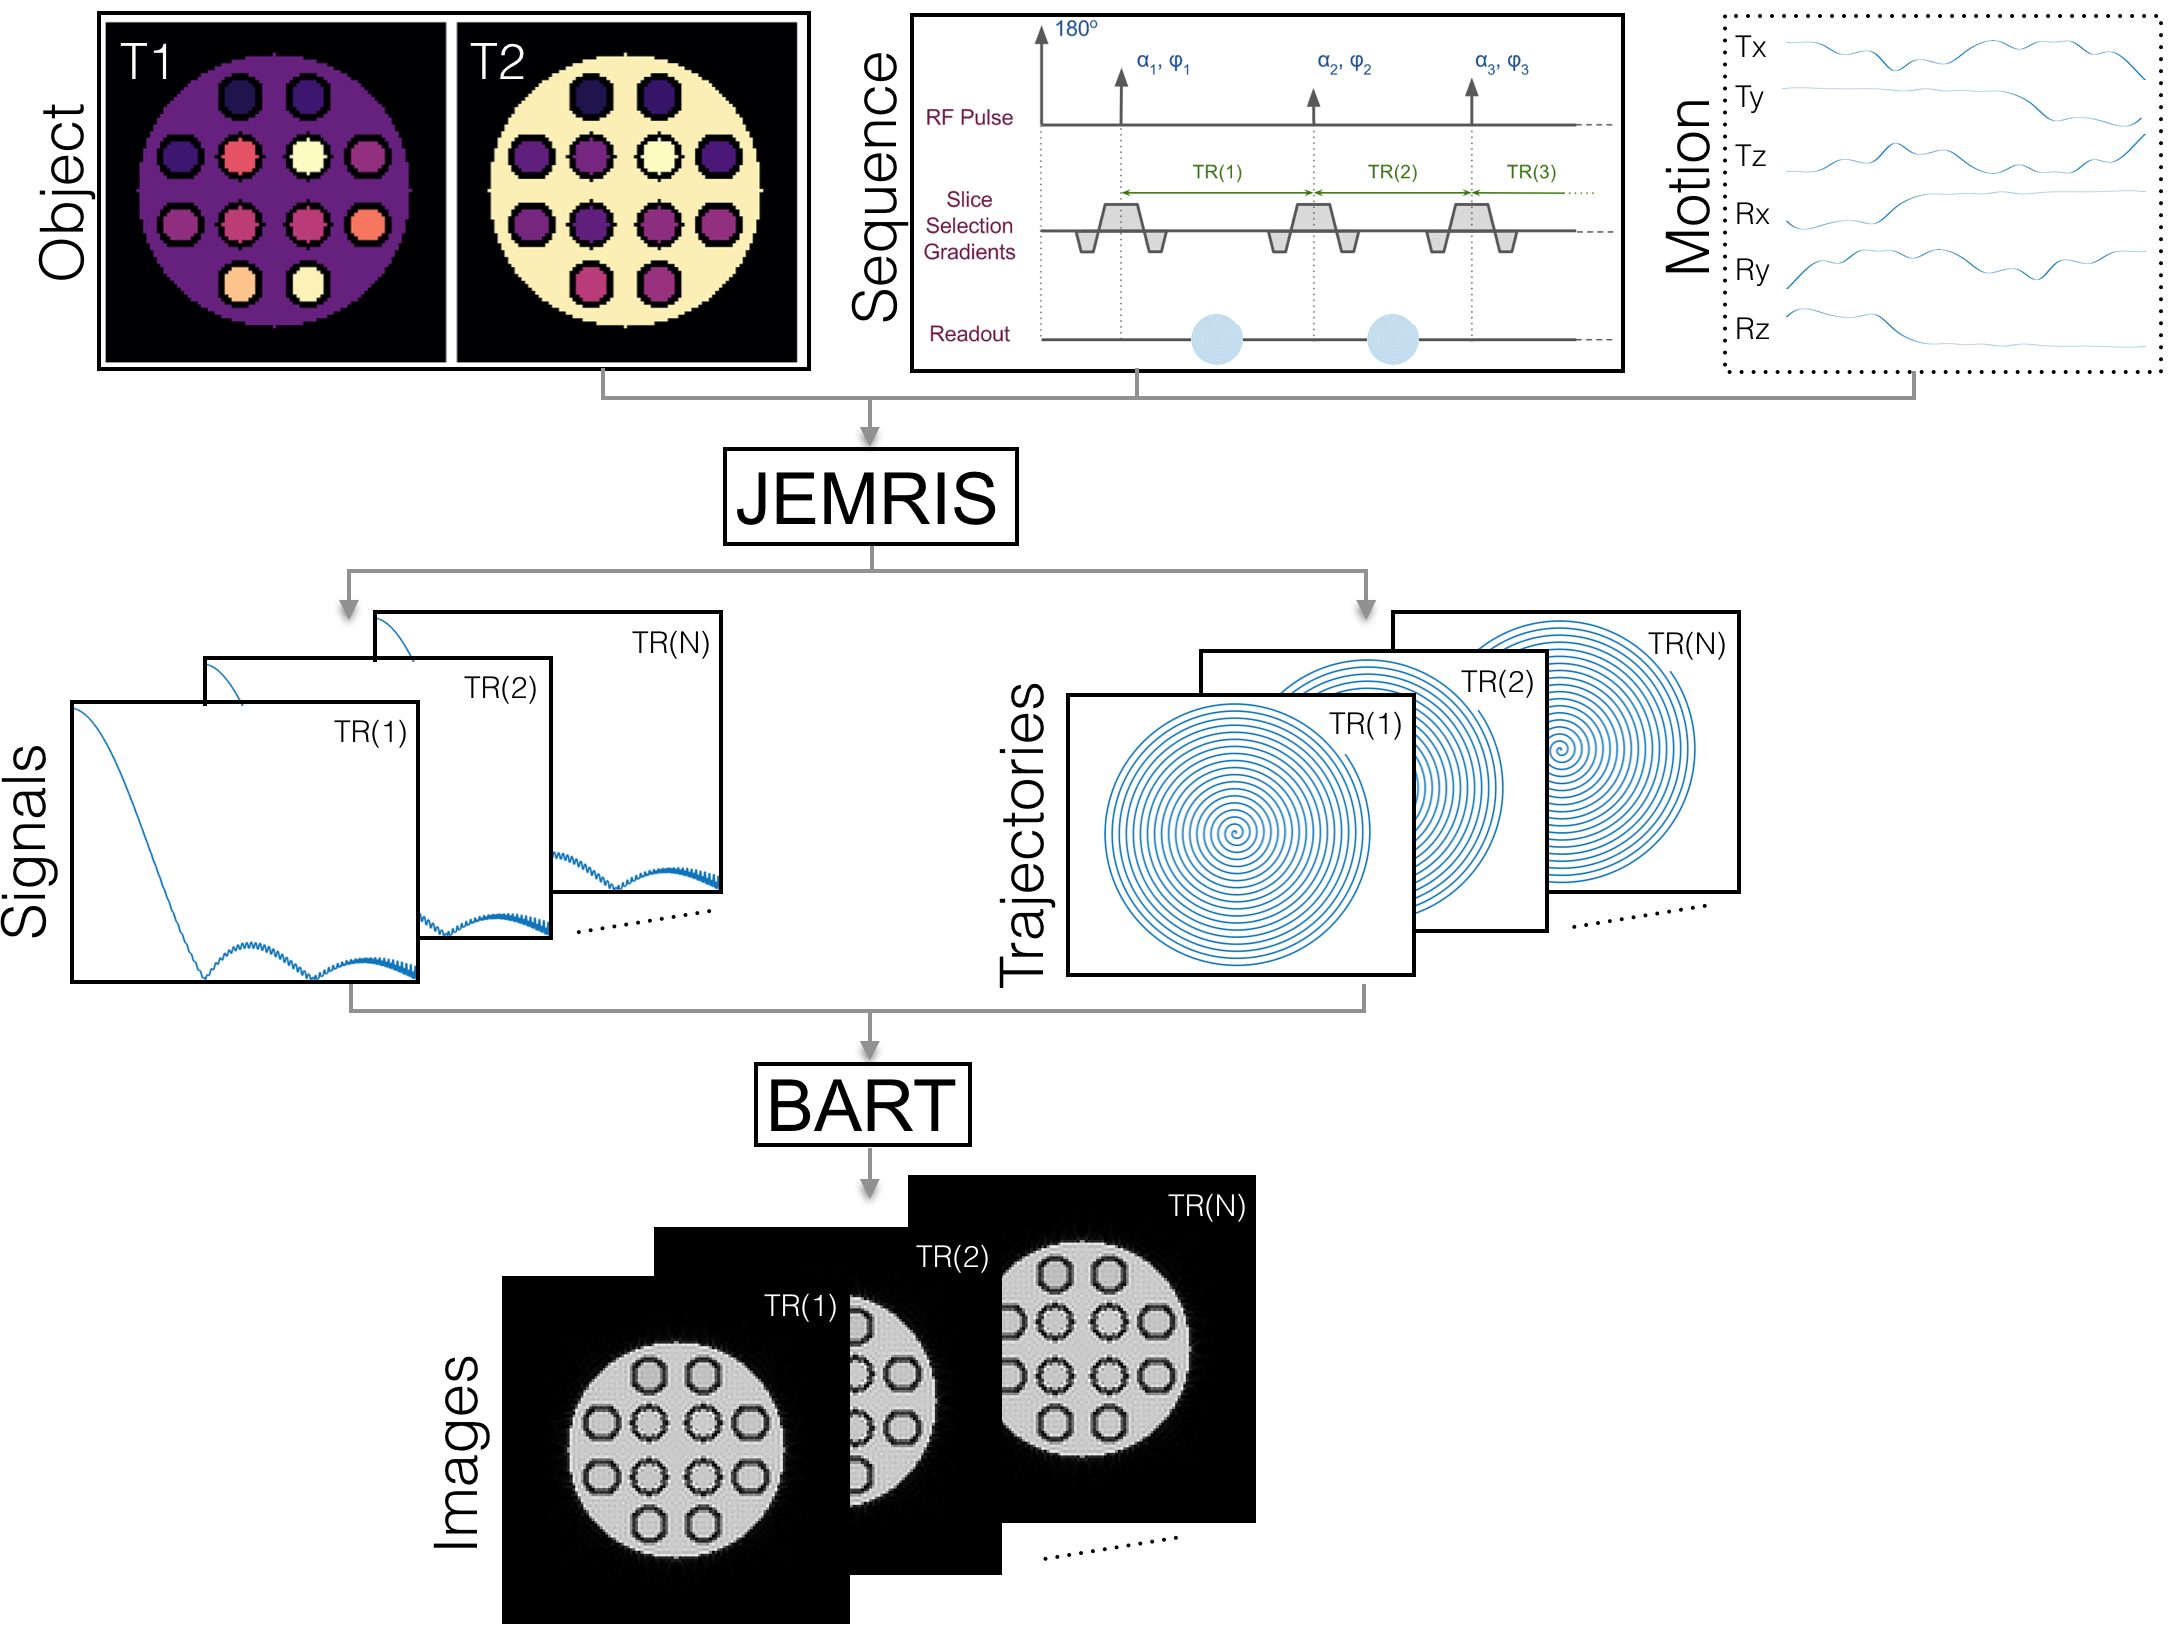
\includegraphics[angle=0,width=1\textwidth, keepaspectratio]{images/mrf/pipelineWithMotion}
%     \caption{Summary of the pipeline used to simulate the images}
%     \label{fig:pipeline}
% \end{figure}

\hfill

% % % % % % % % % % % % % % % % % % % % % % % % % % % % % % % % % % % % % % % % % % % % % % % % % % % % % % % % % % % % % % % % % % % % % % % % % % % % % % % % % % % % % % % % % % % % % % % % % % % % % % % % % % % % % % % % % % % % % % % % % % % % % % % % % % % % % % % % % % % % % % % % 
\subsection{Matching Algorithm}
\label{method:matching}

The pattern matching algorithm used is the same as described in the original MRF implementation \cite{Ma2013}.
It involves a vector dot-product between all the simulated image-space signals and the precomputed dictionary, and the retrieval of the dictionary signal which gives the highest score.
Prior to computing the dot-product, both types of signals are normalised to each having the same sum squared magnitude.
%Conceptually, the two signals need to be as `similar' as possible to say that a certain pair of tissue properties can be attributed to the observed signal.

\hfill

Mathematically, this can be described with the following formulation.
Let there be a dictionary $D \in \mathfrak{C}^{M \times N}$, where M is the number of parameter combinations and N is the number of timepoints.
Any dictionary signal $d_j$, with $j \in [1,M]$, represents the $j^{th}$ row of $D$.
Then, the process of pattern matching involves finding the dictionary entry $d_l$ which satisfies:
\begin{equation}
    d_l = \arg\!\max_{d_j} \, \lvert d_j \, x^* \rvert
\end{equation}
where $x$ is the image-space signal and $x^*$ is the conjugate transpose of $x$.
Both the dictionary entry and the image space signal have to be normalised to have unit length: $\lvert \lvert x \rvert \rvert = \lvert \lvert d_j \rvert \rvert = 1$, where $\lvert \lvert \, \cdot \, \rvert \rvert$ is the Euclidean norm.
Once the match is recovered, the voxel corresponding to the image space signal $x$ is assigned the tissue parameters used to generate the matching entry's signal.

\hfill

This process is then repeated for all the image space signals corresponding to all the voxels in the image dataset.
At the end, a set of tissue parameter maps is created.